\section{Method}
\label{sec:method}
\nothing{In this section, we present our perception-guided neural scene synthesis for virtual reality. \zh{As a real-time overview: we first predict the the color as well as corresponding density for each pixel in the fovea, mid- and far- periphery (or designed 3D point?) given the camera position. Next we apply ray marching to generate the elemental image. Afterwards, we blend the results from each part and tune the contrast for each eye.}\qisun{merged with the following sentences. see if happy}} Based on a concentric spherical representation and trained network predicting RGBDs on the spheres (\Cref{sec:method:representation}), our system predominantly comprises two main steps in real-time: visual-/stereo-acuity adaptive elemental images synthesis with ray marching for fovea, mid-, and far- peripheries; followed by image-based rendering to composite displayed frames (\Cref{sec:synthesis}).
For desired precision-performance balance, we further craft an analytical spatial-temporal model to optimize the determination of our intra-system variables, including coordinates and neural-network parameters (\Cref{sec:method:optimization}).
\begin{figure}
    \centering
    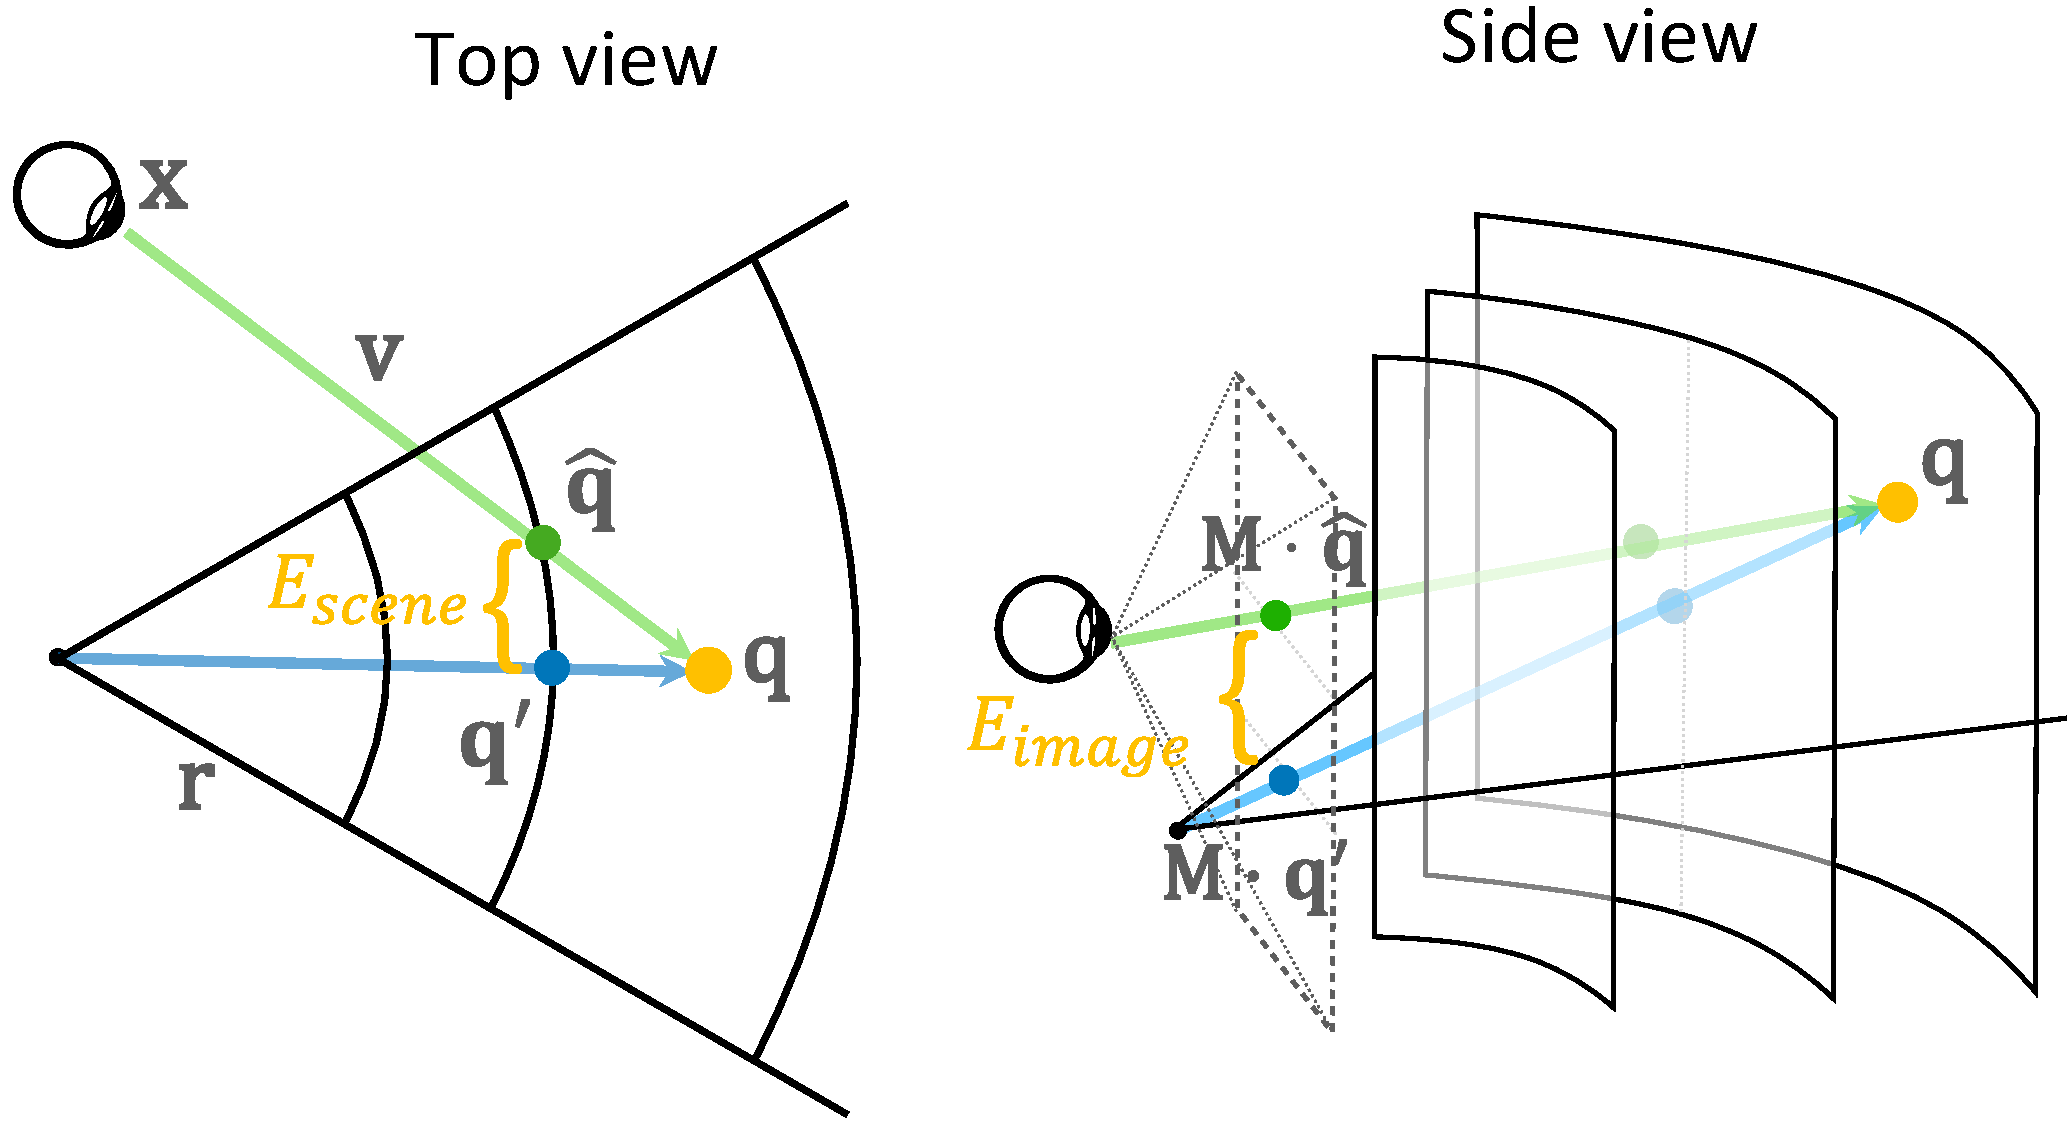
\includegraphics[width=0.96\linewidth]{TOG/figs/parameters.pdf}
    % \subfloat[Notations]{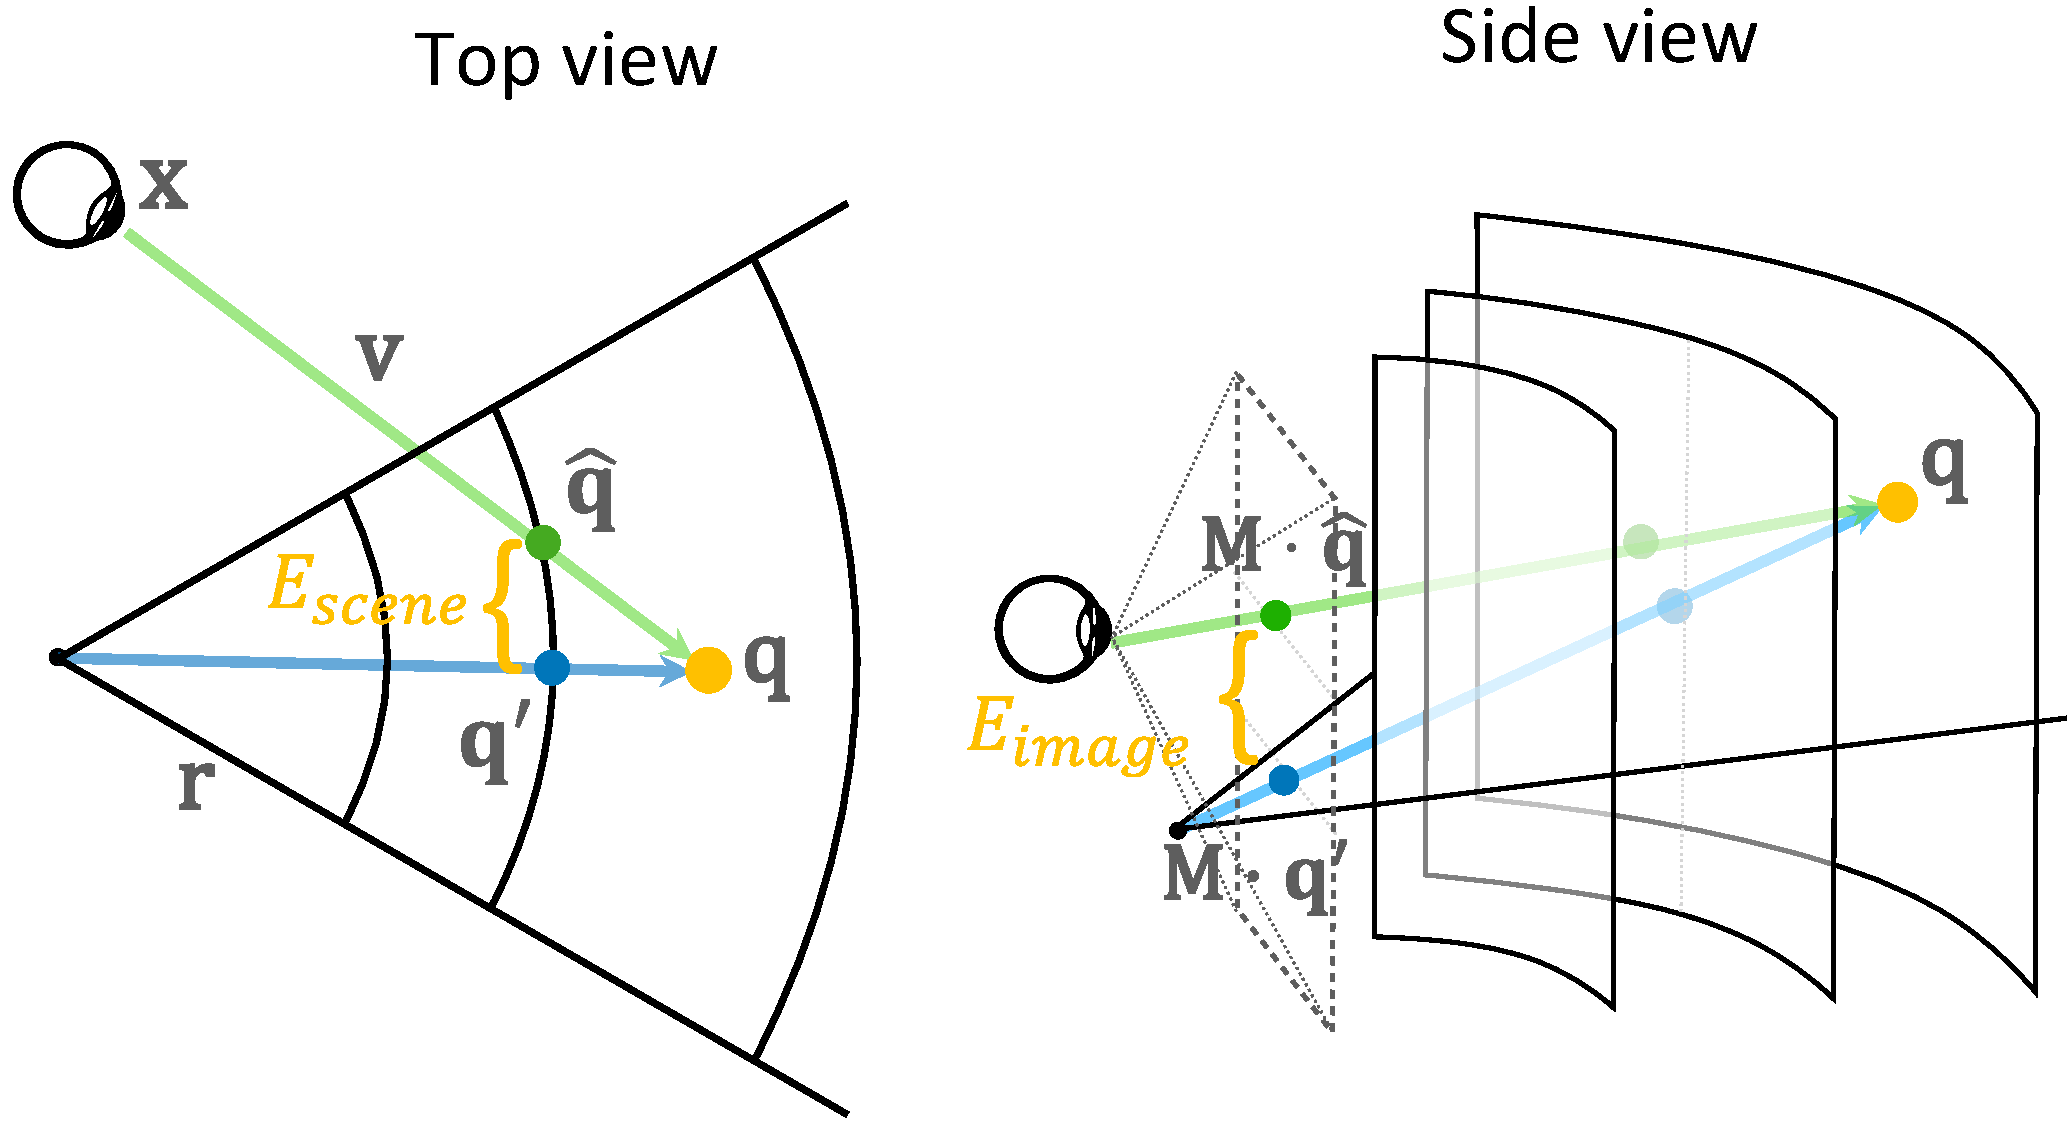
\includegraphics[width=0.96\linewidth]{TOG/figs/parameters.pdf}\label{fig:variables}}
    
    % \subfloat[Correlation between loss and parameters]{\includegraphics[width = 0.96\linewidth]{example-image-a}}
    \Caption{Coordinate system and variable annotations.}
    {%
    We partially visualize our 3D full spherical representation with an example of $\sphereNum=3$ spheres. Variables and equations are annotated at corresponding positions.
    }
    \label{fig:notations}
\end{figure}
\subsection{Egocentric Neural Representation}
\label{sec:method:representation}
The recent single-object-oriented ``outside-in'' view synthesis methods \cite{sitzmann2019deepvoxels,mildenhall2020nerf} typically represent the training targets using uniform voxelization. However, immersive VR environments introduce open challenges for such parameterization due to the rapid variation of the egocentric (first-person) viewing (e.g., \Cref{fig:teaser:scene}).
As a consequence, the neural representation on large virtual environments typically suffer from ghosting artifacts, low resolution, or slow speed (e.g., the white cube and red wall are blurred in \Cref{fig:teaser:latency} and \Cref{fig:teaser:quality}).
%We tailor our method specifically for egocentric (first-person) views in immersive VR environments.
%rendering of immersive viewer-centered ``inside-out'' scenes is challenging owing to the rapid variation of scene content. 
\paragraph{Egocentric coordinates}
To tackle this problem, we are inspired by the recent panorama dis-occlusion methods \cite{Lin:DeepPanorama,Benjamin:2020:RTV,Broxton:immersiveLF} to depict the rapidly varying first-person views with concentric spherical coordinates. This representation enables robust rendering at real-time rates and allows for 6DoF interaction to navigate complex immersive environments. 
As visualized in \Cref{fig:notations}, our representation is parameterized with the number of concentric spheres ($\sphereNum$) and their respective radii ($\mathbf{\sphereRadius}=\{\sphereRadius_i\},i\in [1,\sphereNum]$). Our network aims at predicting the function $\mlpFunc(\hat{\SpatialPt})\triangleq(r,g,b,d)$ of any position $\mathbf{\hat{\SpatialPt}}({\sphereRadius_{i,i\in[1,\sphereNum]},\theta,\phi})$ on these $\sphereNum$ spherical surfaces. %\dnc{$\mathbf{q}$ may be more proper}\qisun{Just to avoid confusion with \Cref{fig:notations}. What do you think?}\dnc{Then perhaps we can use $\hat{q}$ as shown in \Cref{fig:notations} I think the alphabet 'q' means it's in spherical system, 'p' never exists anywhere else}
%\zh{considering denoting $\sphereNum$ and $\mathbf{\sphereRadius}=\{\sphereRadius_i\},i\in [1,\sphereNum]$ in \Cref{fig:notations}}
Here, $(r,g,b)$ and $d$ are the predicted color and density, respectively. 
We then employ a ray marching through this intermediate function to produce images of specified views.

\paragraph{Training and synthesis}
%\dnc{Perhaps we can merge this paragraph with above section? And move the last paragraph of above section to here as a intro. Then this section is more focusing on GAZE-AWARE}
For each scene, we approximate the function $\mlpFunc$ by a multilayer perceptron (MLP) network, similar to \cite{mildenhall2020nerf}.
The network is composed of $\mlpLayerNum$ fully-connected layers of $\mlpChannelNum$ channels, each using ReLu as the activation function. We further determine $\mlpLayerNum$, $\mlpChannelNum$ and $\sphereNum$ via a spatial-temporal optimization in \Cref{sec:method:optimization}.
Given rays of pixels in an image, the network predicts the colors and densities along these rays on every sphere. The ray marching weighted integrates predictions in back-to-front order to obtain actual colors of corresponding pixels.% based on users' frame-wise views. 
Similar to \cite{mildenhall2020nerf}, we apply a trigonometric input encoding and compute the L2-distance between the volume-rendered and mesh-rendered images as the training loss function. We discuss the specifics of training data creation and implementations in \Cref{sec:impl}.\nothing{\zh{Considering removing the last sentence. I think it is clear that this paragraph is not about details, guess reviewers are not expected to see the details. Or we should lead them not to expect details here.}}

\subsection{Gaze-Aware Synthesis}
\label{sec:synthesis}
\qisun{@nianchen: does this section title sounds reasonable to you?}
%The scene representation above is created to parameterize a given 3D space for neural synthesis. 
%the foveated rendering manner of VR display through training two orthogonal neural networks that are tailored for the perceptual acuity variances.
%\zh{shall we explicitly name the representation with exactly `concentric spherical coordinate system' earlier?}
Our concentric spherical coordinate, as described in \Cref{sec:method:representation}, addresses the view variance problem in VR. However, it still suffers from significant rendering latency (several seconds per frame). This is one of the core challenges causing neural representation to be unsuitable yet for VR. Instead of the typical single image prediction, we synthesize multiple elemental images to enable real-time responsiveness.
The elemental images are generated based on the viewer's head and gaze motions and are adapted to the retinal acuity in resolution and stereo. %We detail our network design and elemental image synthesis in the following section. %We enable real-time responsiveness via introducing gaze-adaptive synthesis mechanisms.
\begin{figure}[b]
    \centering
    \subfloat[fovea]{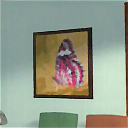
\includegraphics[width=0.3\linewidth]{TOG/figs/layer_blend/lobby_view0000_fovea.png}\label{fig:system:fovea}}\hspace{1em}
    \subfloat[mid-periphery]{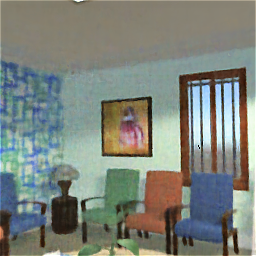
\includegraphics[width=0.3\linewidth]{TOG/figs/layer_blend/lobby_view0000_mid.png}\label{fig:system:mid}}\hspace{1em}
    \subfloat[far-periphery]{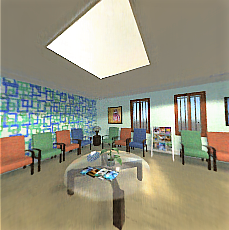
\includegraphics[width=0.3\linewidth]{TOG/figs/layer_blend/lobby_view0000_periph.png}\label{fig:system:far}}
    
    \subfloat[display image]{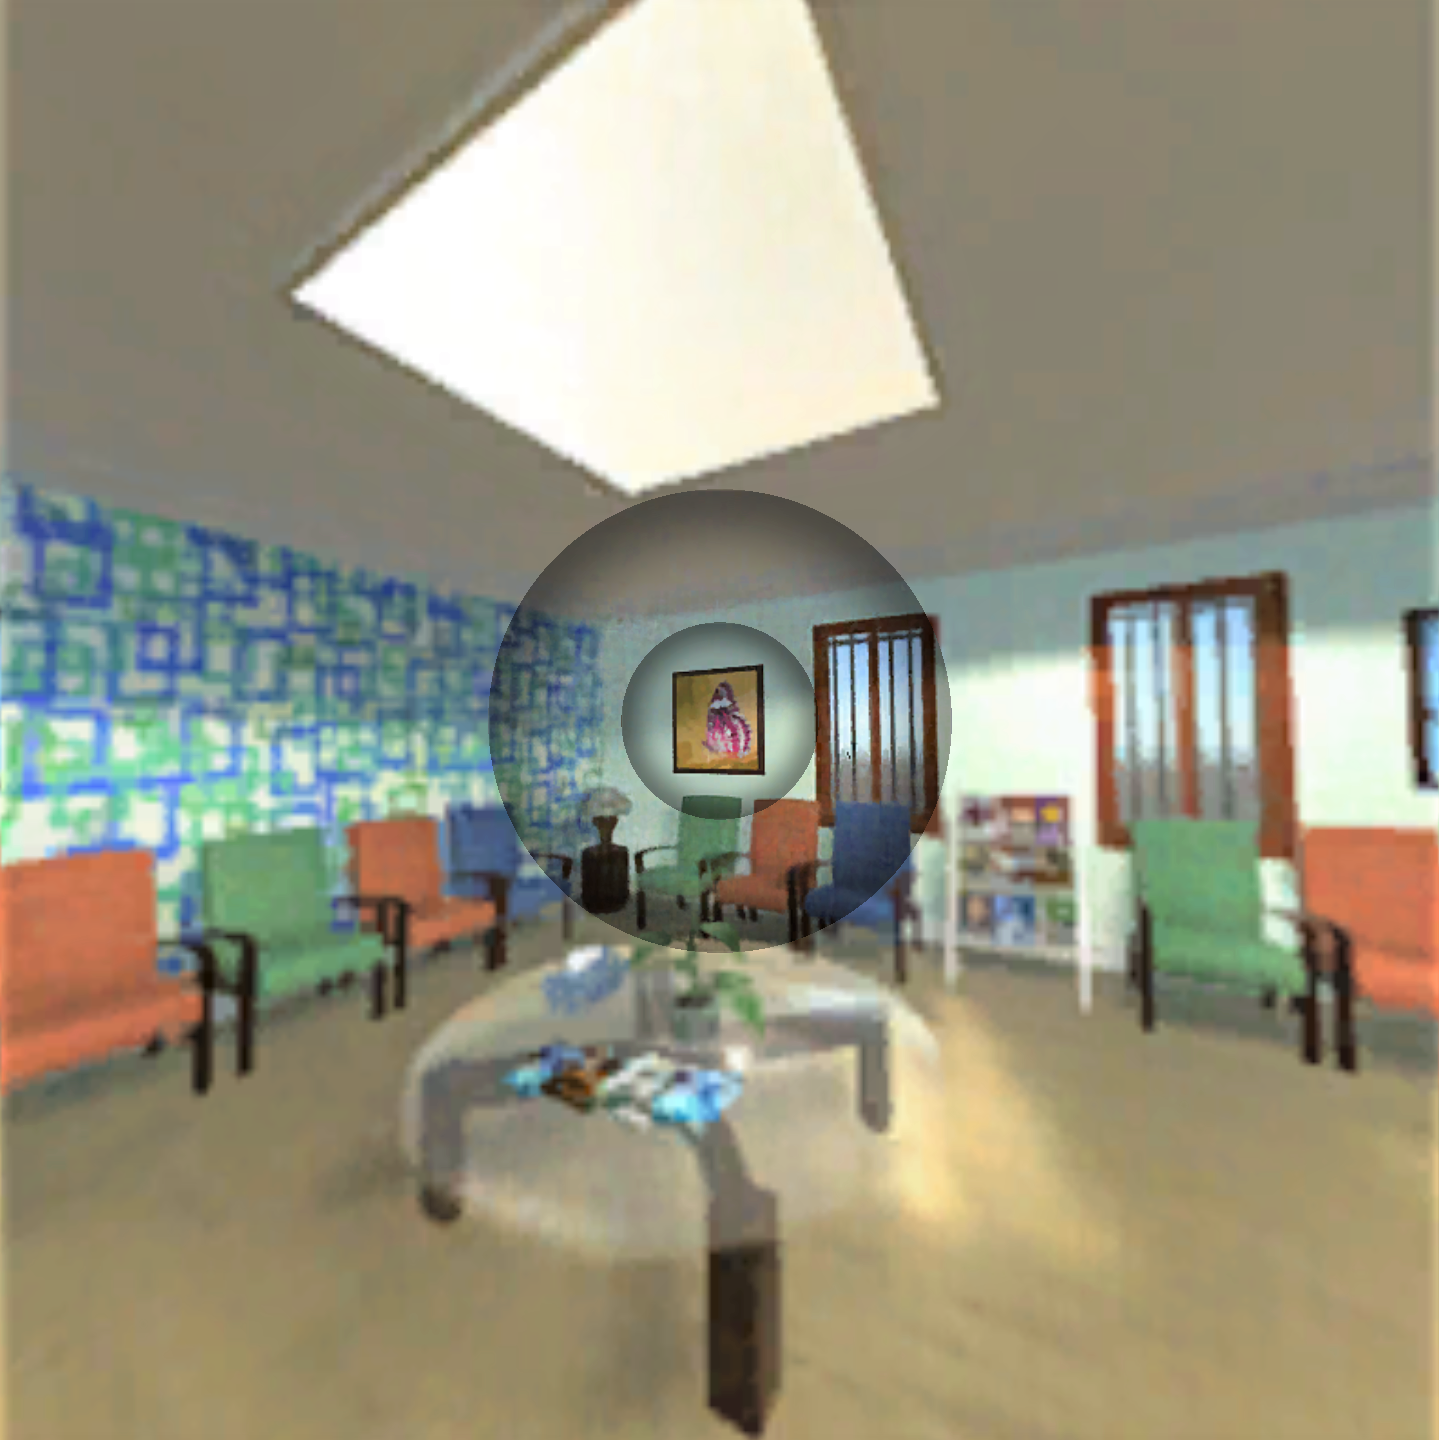
\includegraphics[width=0.9\linewidth]{TOG/figs/layer_blend/lobby_view0000_blendmask.png}\label{fig:system:blending}}
    \Caption{Visual acuity adaptive synthesis and rendering mechanism.}
    {%
    \subref{fig:system:fovea}/\subref{fig:system:mid}/\subref{fig:system:far} shows our individual gaze-contingent synthesis for fovea (within $20$ deg)/mid-periphery (within $45$ deg)/far-periphery (within $110$ deg, the capability of our VR display), respectively. 
    \subref{fig:system:blending} illustrates our real-time rendering system by dynamically blending the individual images to the final displayed frame.
    }
    \label{fig:system}
\end{figure}
\subsubsection{Adaptive visual acuity}
% The human vision is foveated. With the high field-of-view VR displays, we exploit the spatially-adaptive visual acuity to significantly accelerate the computation without compromising {\it perceptual} quality.
The human vision is foveated. Inspired by this, we significantly accelerate the computation by integrating the characteristic of spatially-adaptive visual acuity without compromising {\it perceptual} quality.

Specifically, given device-tracked camera position ($\rayo$), direction ($\camDir$), and gaze position ($\gazeDir$),
we train two orthogonal networks (i.e., function $\mlpFunc$s) to synthesize foveal ($\imageFoveal(\rayo,\camDir,\gazeDir)$, $0-20$ deg), and peripheral elemental images (i.e., two $\mlpFunc$s to deploy for ray marching) for each eye. 
The periphery includes mid- ($\imageMid(\rayo,\camDir,\gazeDir)$, $0-45$ deg) and high- eccentricity visual fields ($\imageFar(\rayo,\camDir$), $0-110$ deg), see \Cref{fig:system}.
Note that $\imageFar$ is independent from the gaze direction $\gazeDir$. 
%The images are defined as functions that maps individual camera rays ($\rayo,\rayd$) to an RGB color.
Specifically, to incorporate the display capabilities and perceptual effects, we define $\imageFoveal$/$\imageMid$/$\imageFar$ as of $128^2$/$256^2$/$230\times256$ resolutions respectively.
That is, the $\imageFoveal$ has the highest spatial resolution of $6.4$ pixels per degree (PPD), higher than those of $\imageMid$ ($5.7$ PPD) and $\imageFar$ ($2.33$ PPD).
%In each frame, the two networks independently return three elemental images, as seen from the separation range in deg, gradually larger areas along eccentricity. An example is shown in \Cref{fig:system}.
% ZH: add conclusive or ending sentences here.
%In each frame, the two networks independently return three elemental images, as seen from the separation range in deg, gradually larger areas along eccentricity. An example is shown in \Cref{fig:system}.
% ZH: add conclusion or ending sentences here.

\subsubsection{Adaptive stereo-acuity}
Head-mounted VR displays require stereo rendering, thus the elemental images $\imageFoveal^{\{l,r\}}$, $\imageMid^{\{l,r\}}$, and $\imageFar^{\{l,r\}}$ for each ($l$eft and $r$ight) eye. This, however, doubles the inference computation cost that is critical for latency- and frame-rate- sensitive VR experience 
\nothing{The separation of the three elemental images considers the varied visual acuity. However, in a head-mounted stereo VR displays, the rendered image are for two eyes, resulting in double computation for $\imageFoveal^{\{l,r\}}$, $\imageMid^{\{l,r\}}$, and $\imageFar^{\{l,r\}}$. Here $l$ and $r$ represent the projection images for left ($\rayo^l$) and right ($\rayo^r$) eyes respectively. 
Whereas, because $\imageMid^{\{l,r\}}$ and $\imageFar^{\{l,r\}}$ demand high spatial resolution due to their large eccentricity coverage, }
(please refer to \Cref{sec:study:intra} for breakdown comparisons).

To further accelerate stereo rendering towards real-time experience, we accommodate the inference process with the adaptive stereo-acuity in the periphery.
In fact, besides the visual acuity, psychophysical studies have also revealed human's significantly declined stereopsis while receding from the gaze point \cite{mochizuki2012magnitude}. Inspired by this characteristic, we perform the computation with $\imageFoveal^{\{l,r\}}$, $\imageMid^c$, and $\imageFar^c$ instead of inferring $6$ elemental images, where $c$ indicates the view at the central eye (the midpoint of the left and right eyes). \Cref{fig:mono} visualizes the stereopsis changes from the adaptation using an anaglyph. 
\begin{figure}[tbh]
    \centering
    %\subfloat[w/o gaze-adaptive stereo]{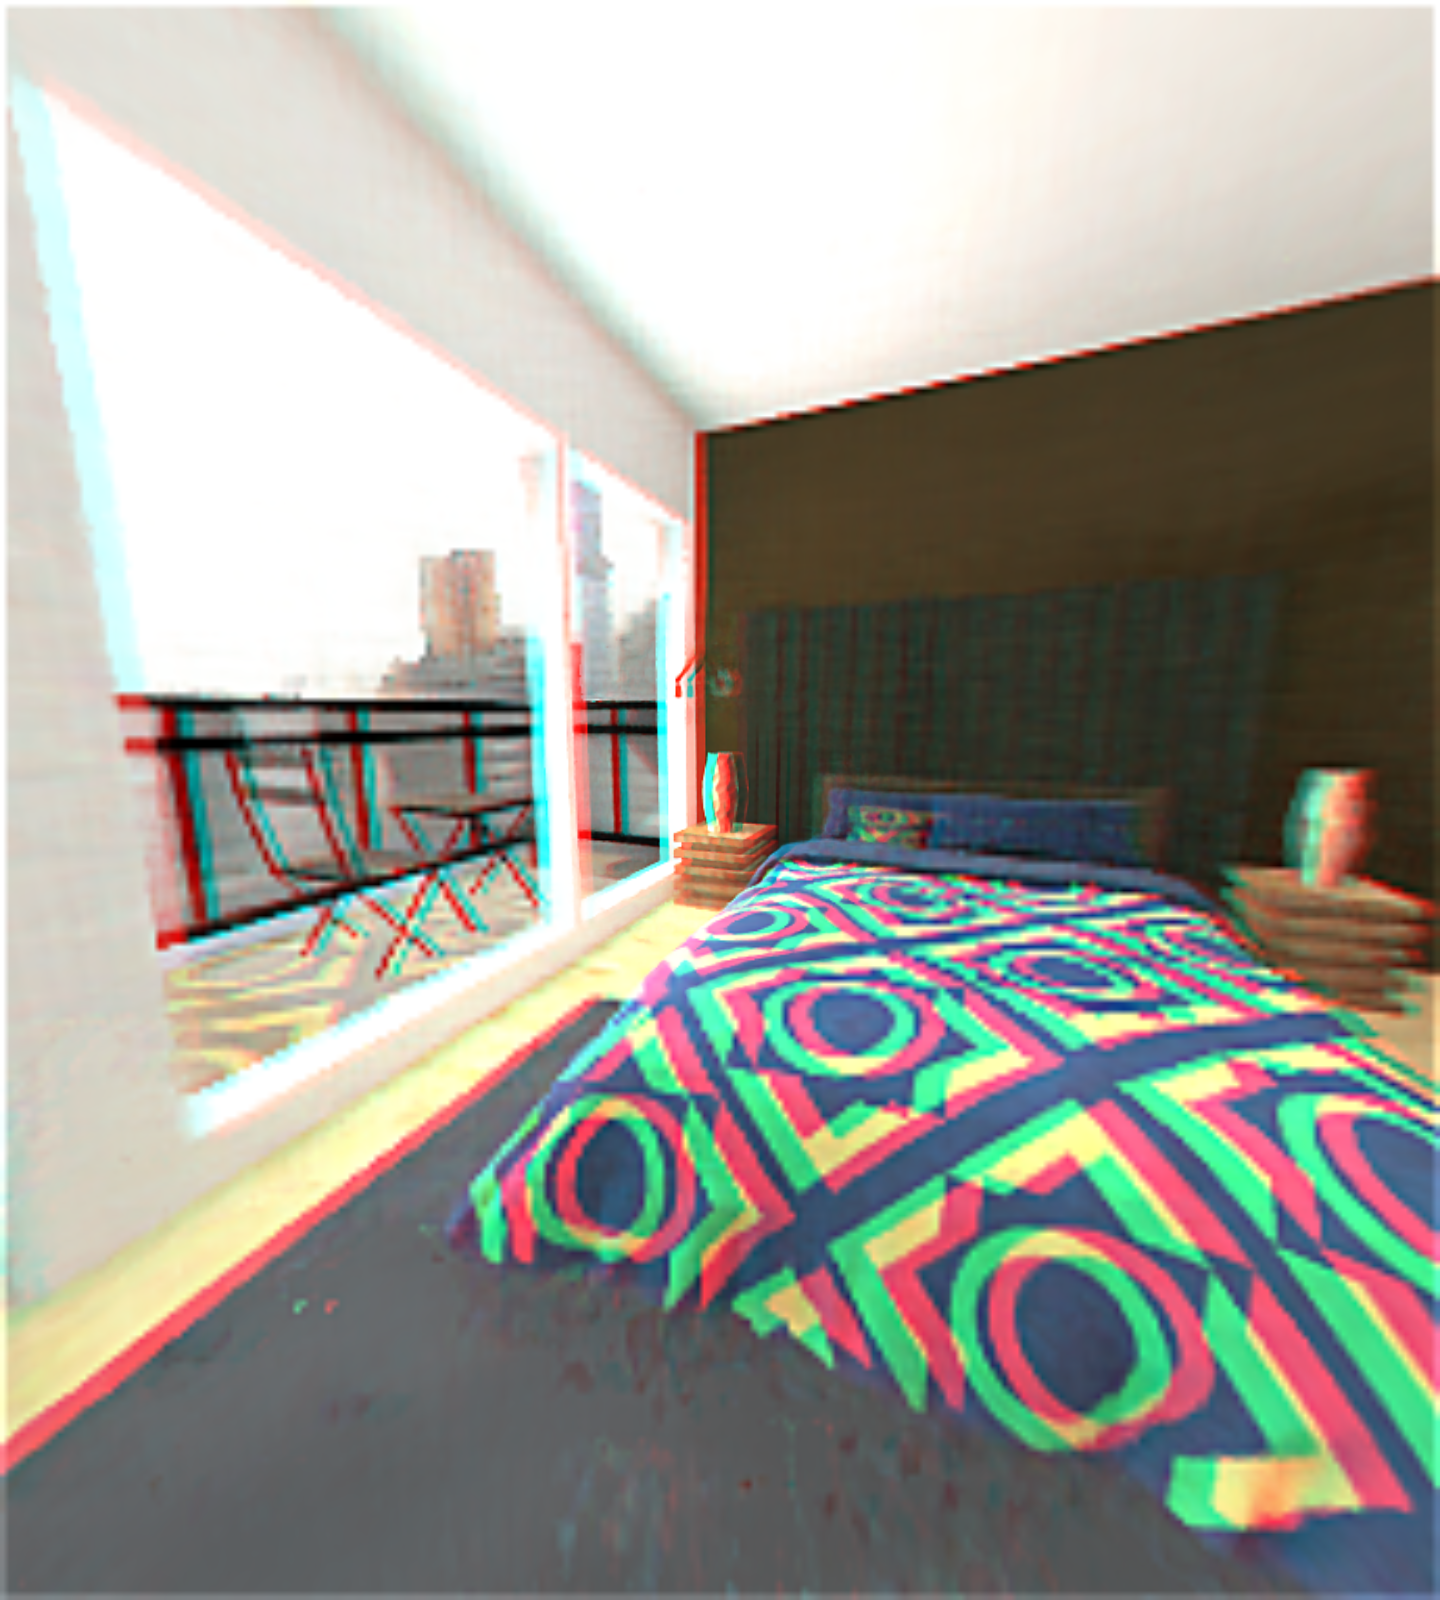
\includegraphics[width=0.248\linewidth]{TOG/figs/stereo_periphery/bedroom_view0000_blended_stereo.png}\label{fig:mono:wo}}
    %\subfloat[w/ gaze-adaptive stereo]{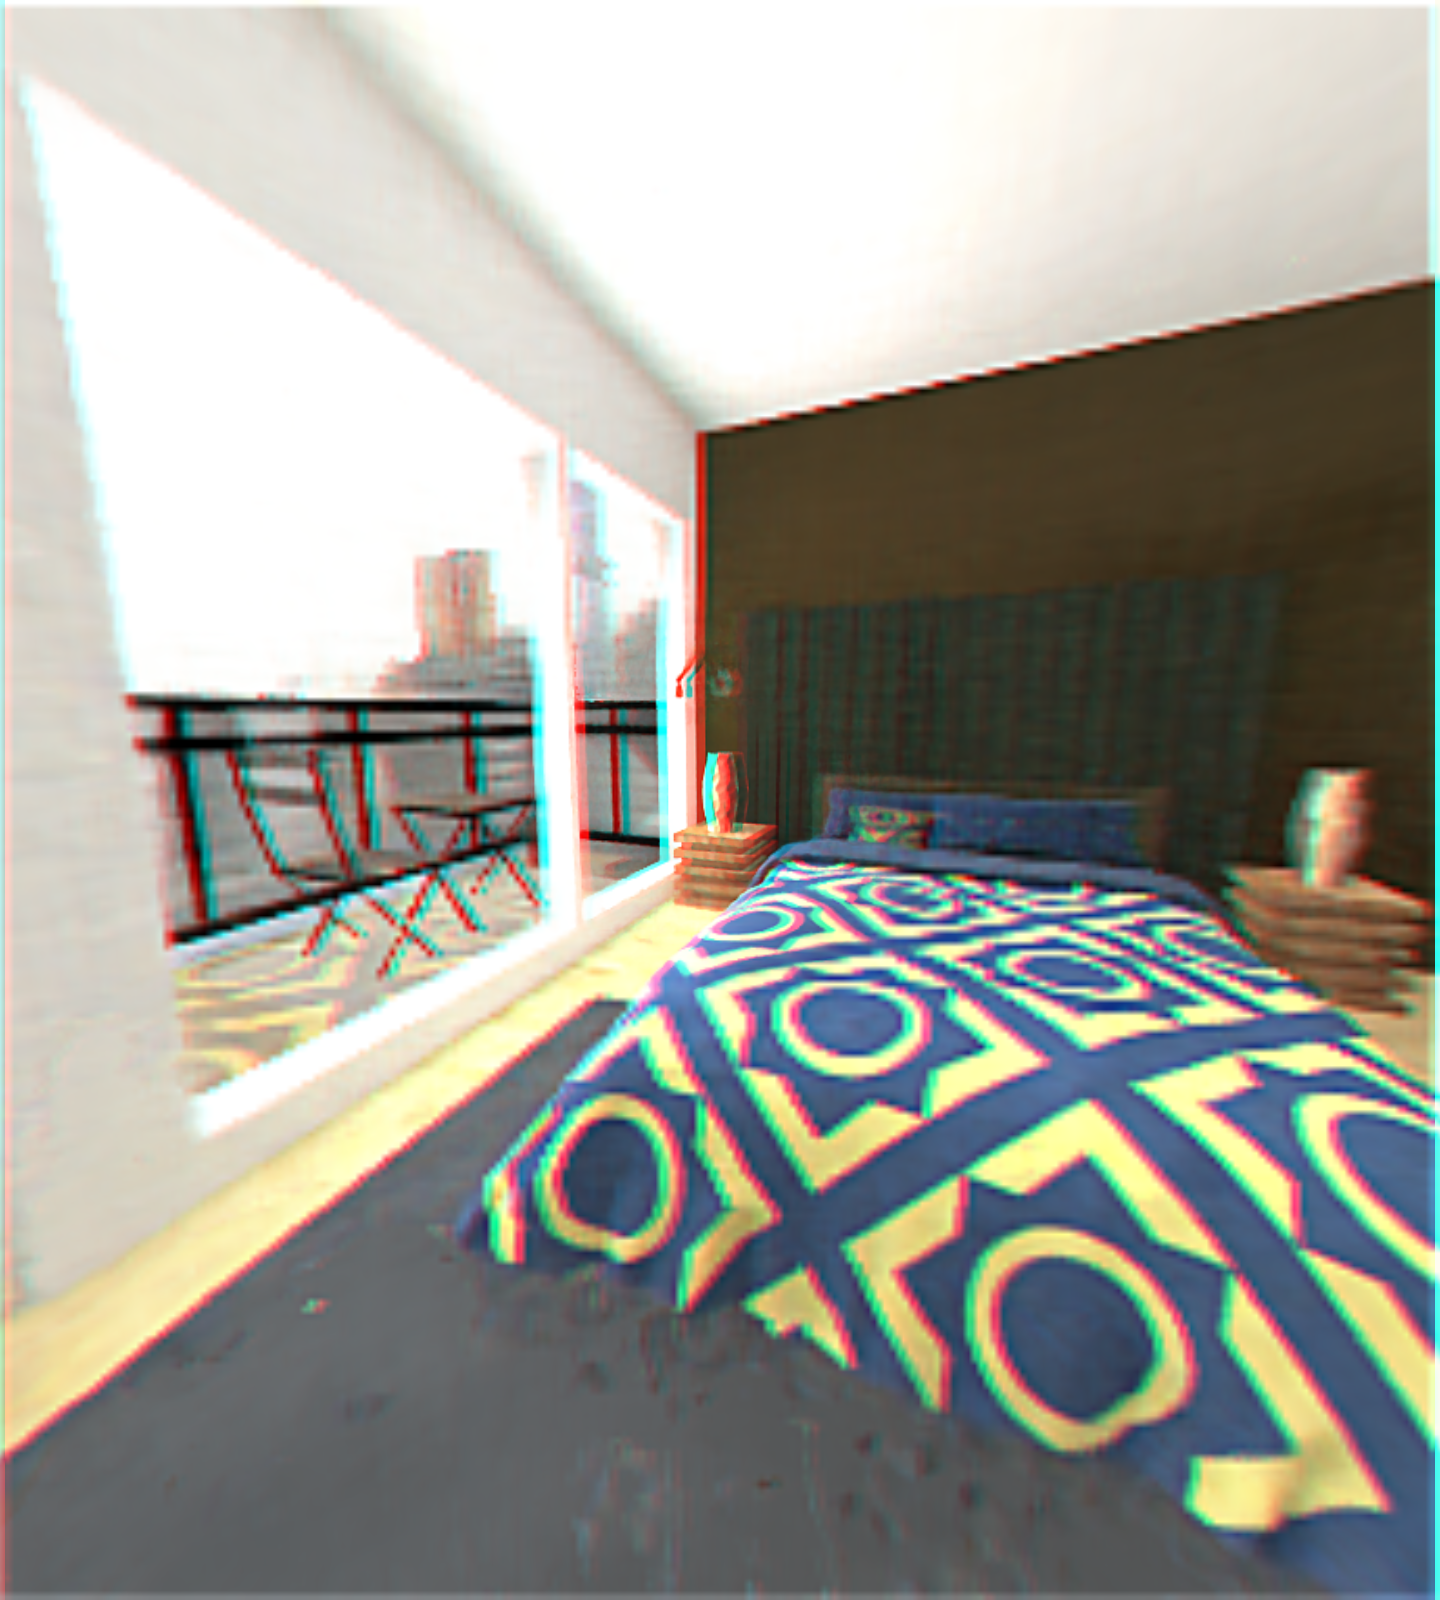
\includegraphics[width=0.248\linewidth]{TOG/figs/mono_periphery/bedroom_view0000_blended_stereo.png}%\label{fig:mono:w}}
    %\subfloat[w/o gaze-adaptive stereo]{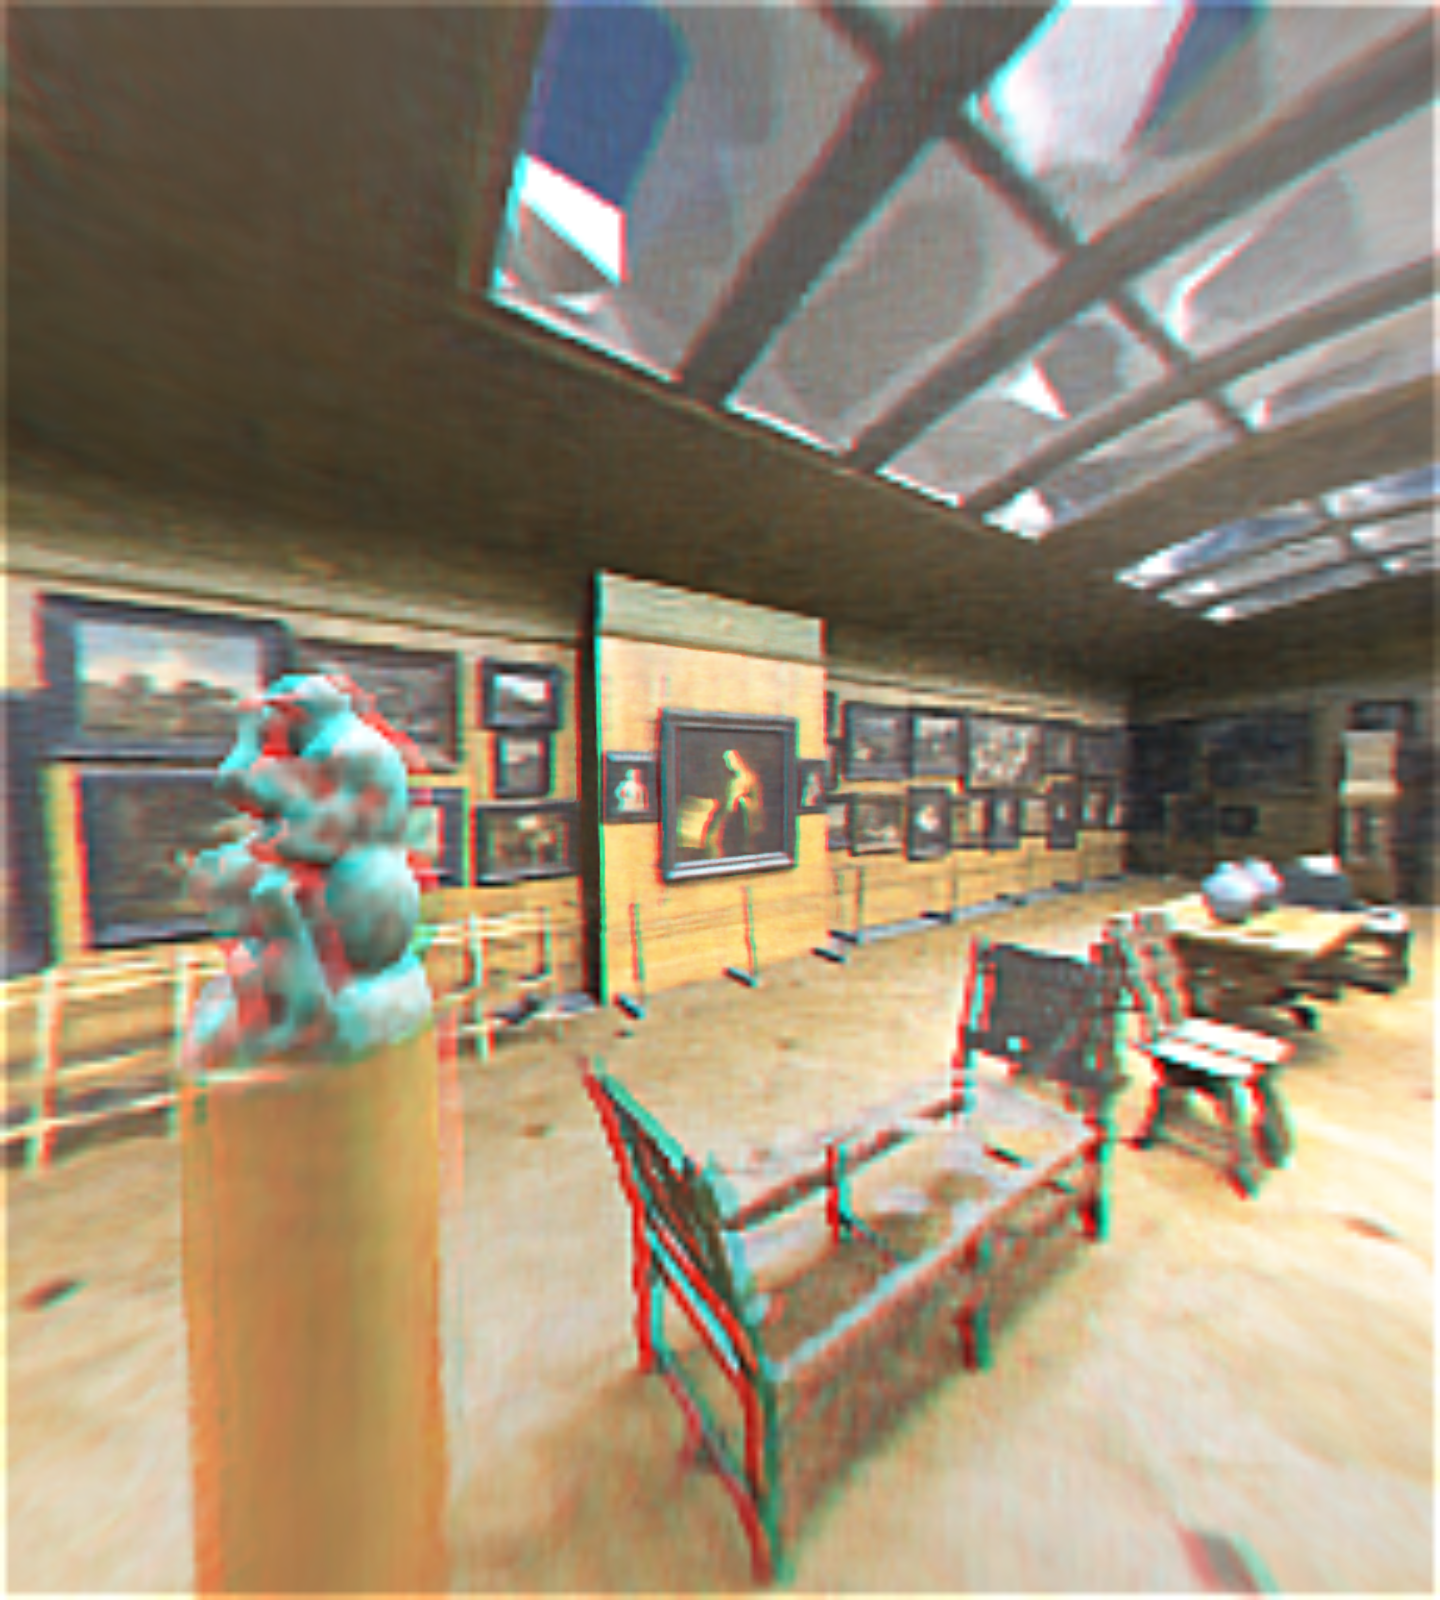
\includegraphics[width=0.248\linewidth]{TOG/figs/stereo_periphery/gallery_view0000_blended_stereo.png}\label{fig:mono:wo}}
    %\subfloat[w/ gaze-adaptive stereo]{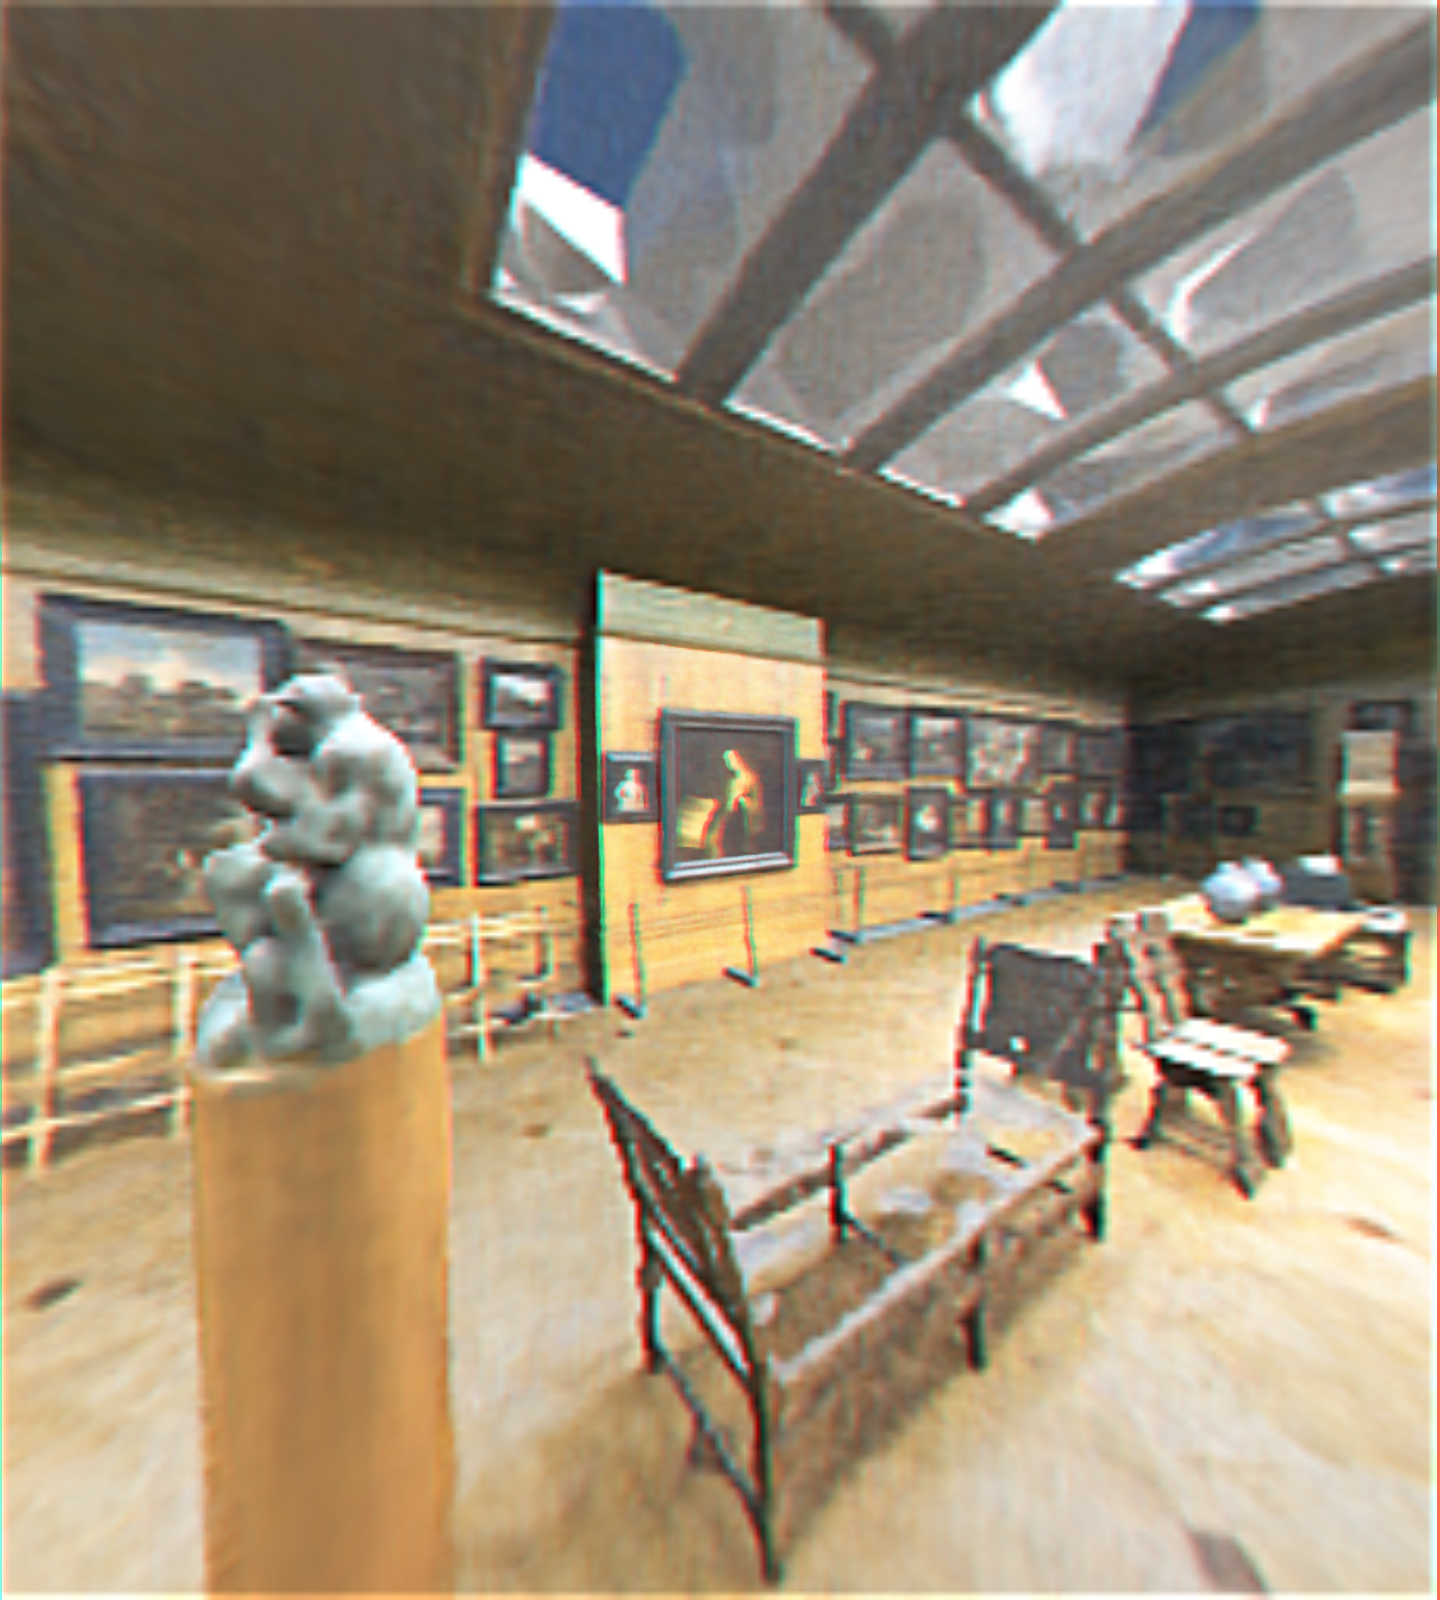
\includegraphics[width=0.248\linewidth]{TOG/figs/mono_periphery/gallery_view0000_blended_stereo.png}%\label{fig:mono:w}}
    
    \subfloat[w/o gaze-adaptive stereo]{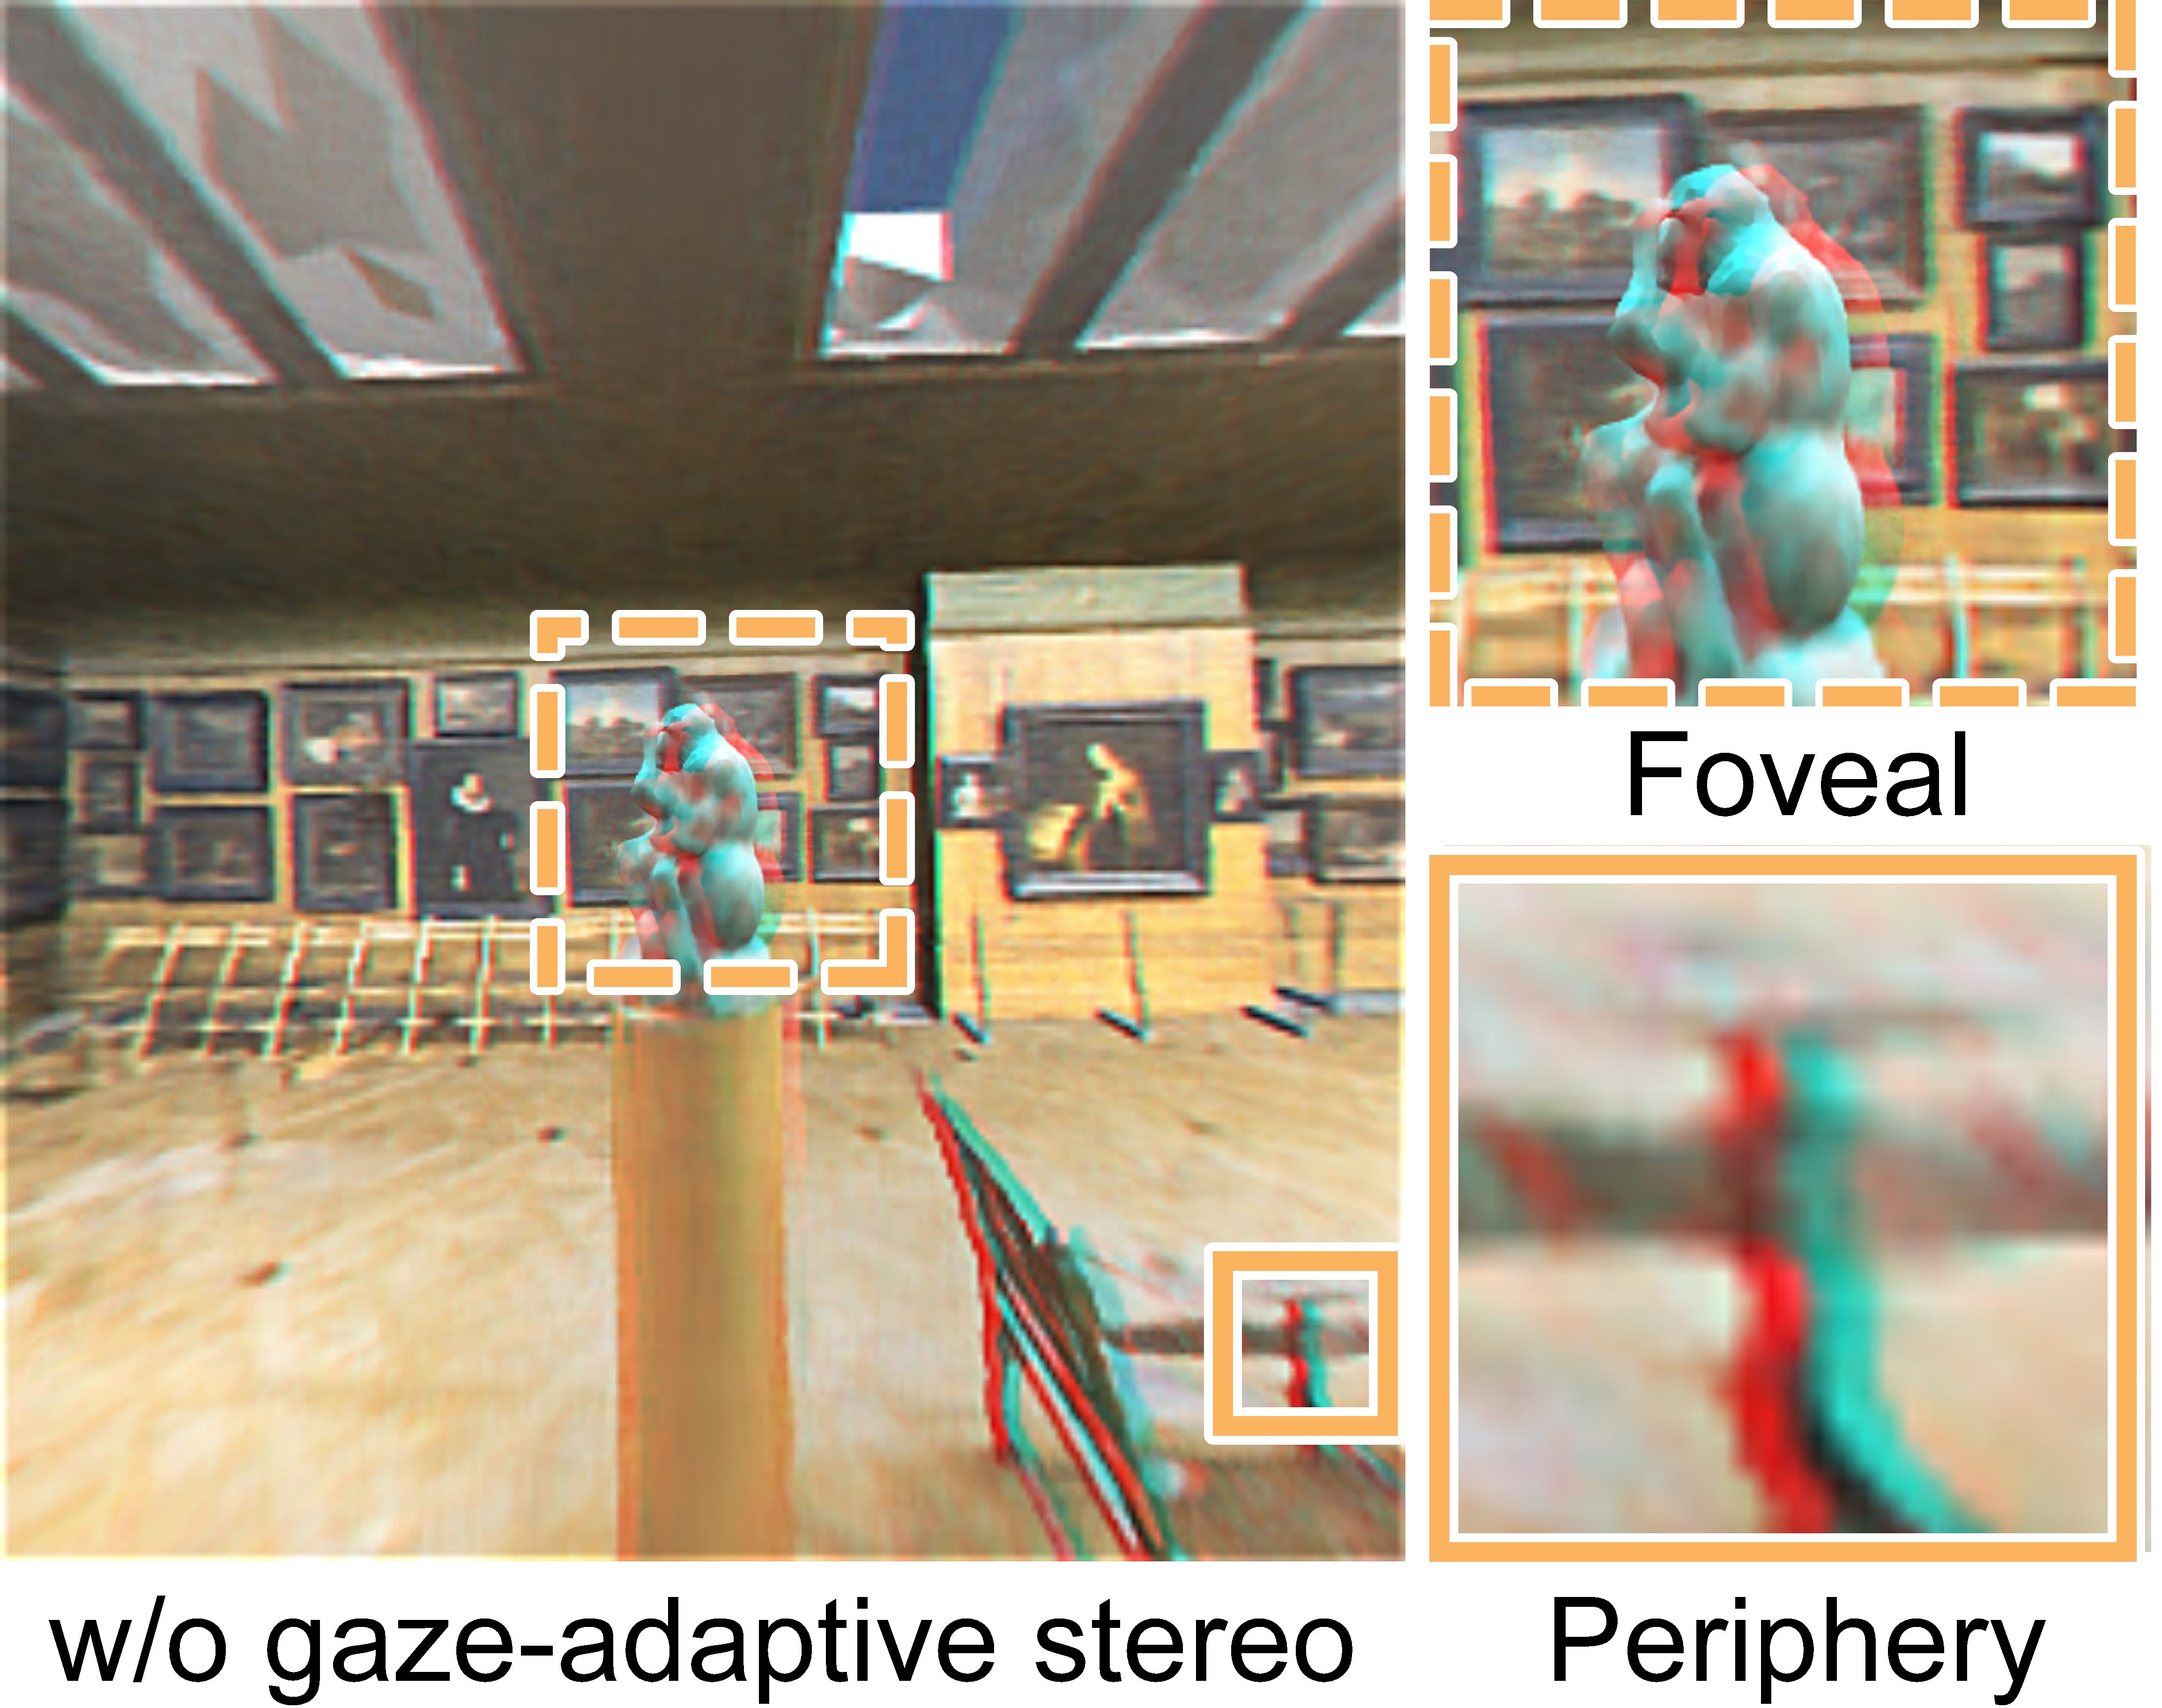
\includegraphics[width=0.48\linewidth]{TOG/figs/stereo_periphery/stereo_periphery.pdf}\label{fig:mono:wo}}%\hspace{0.5em}
    \subfloat[w/ gaze-adaptive stereo]{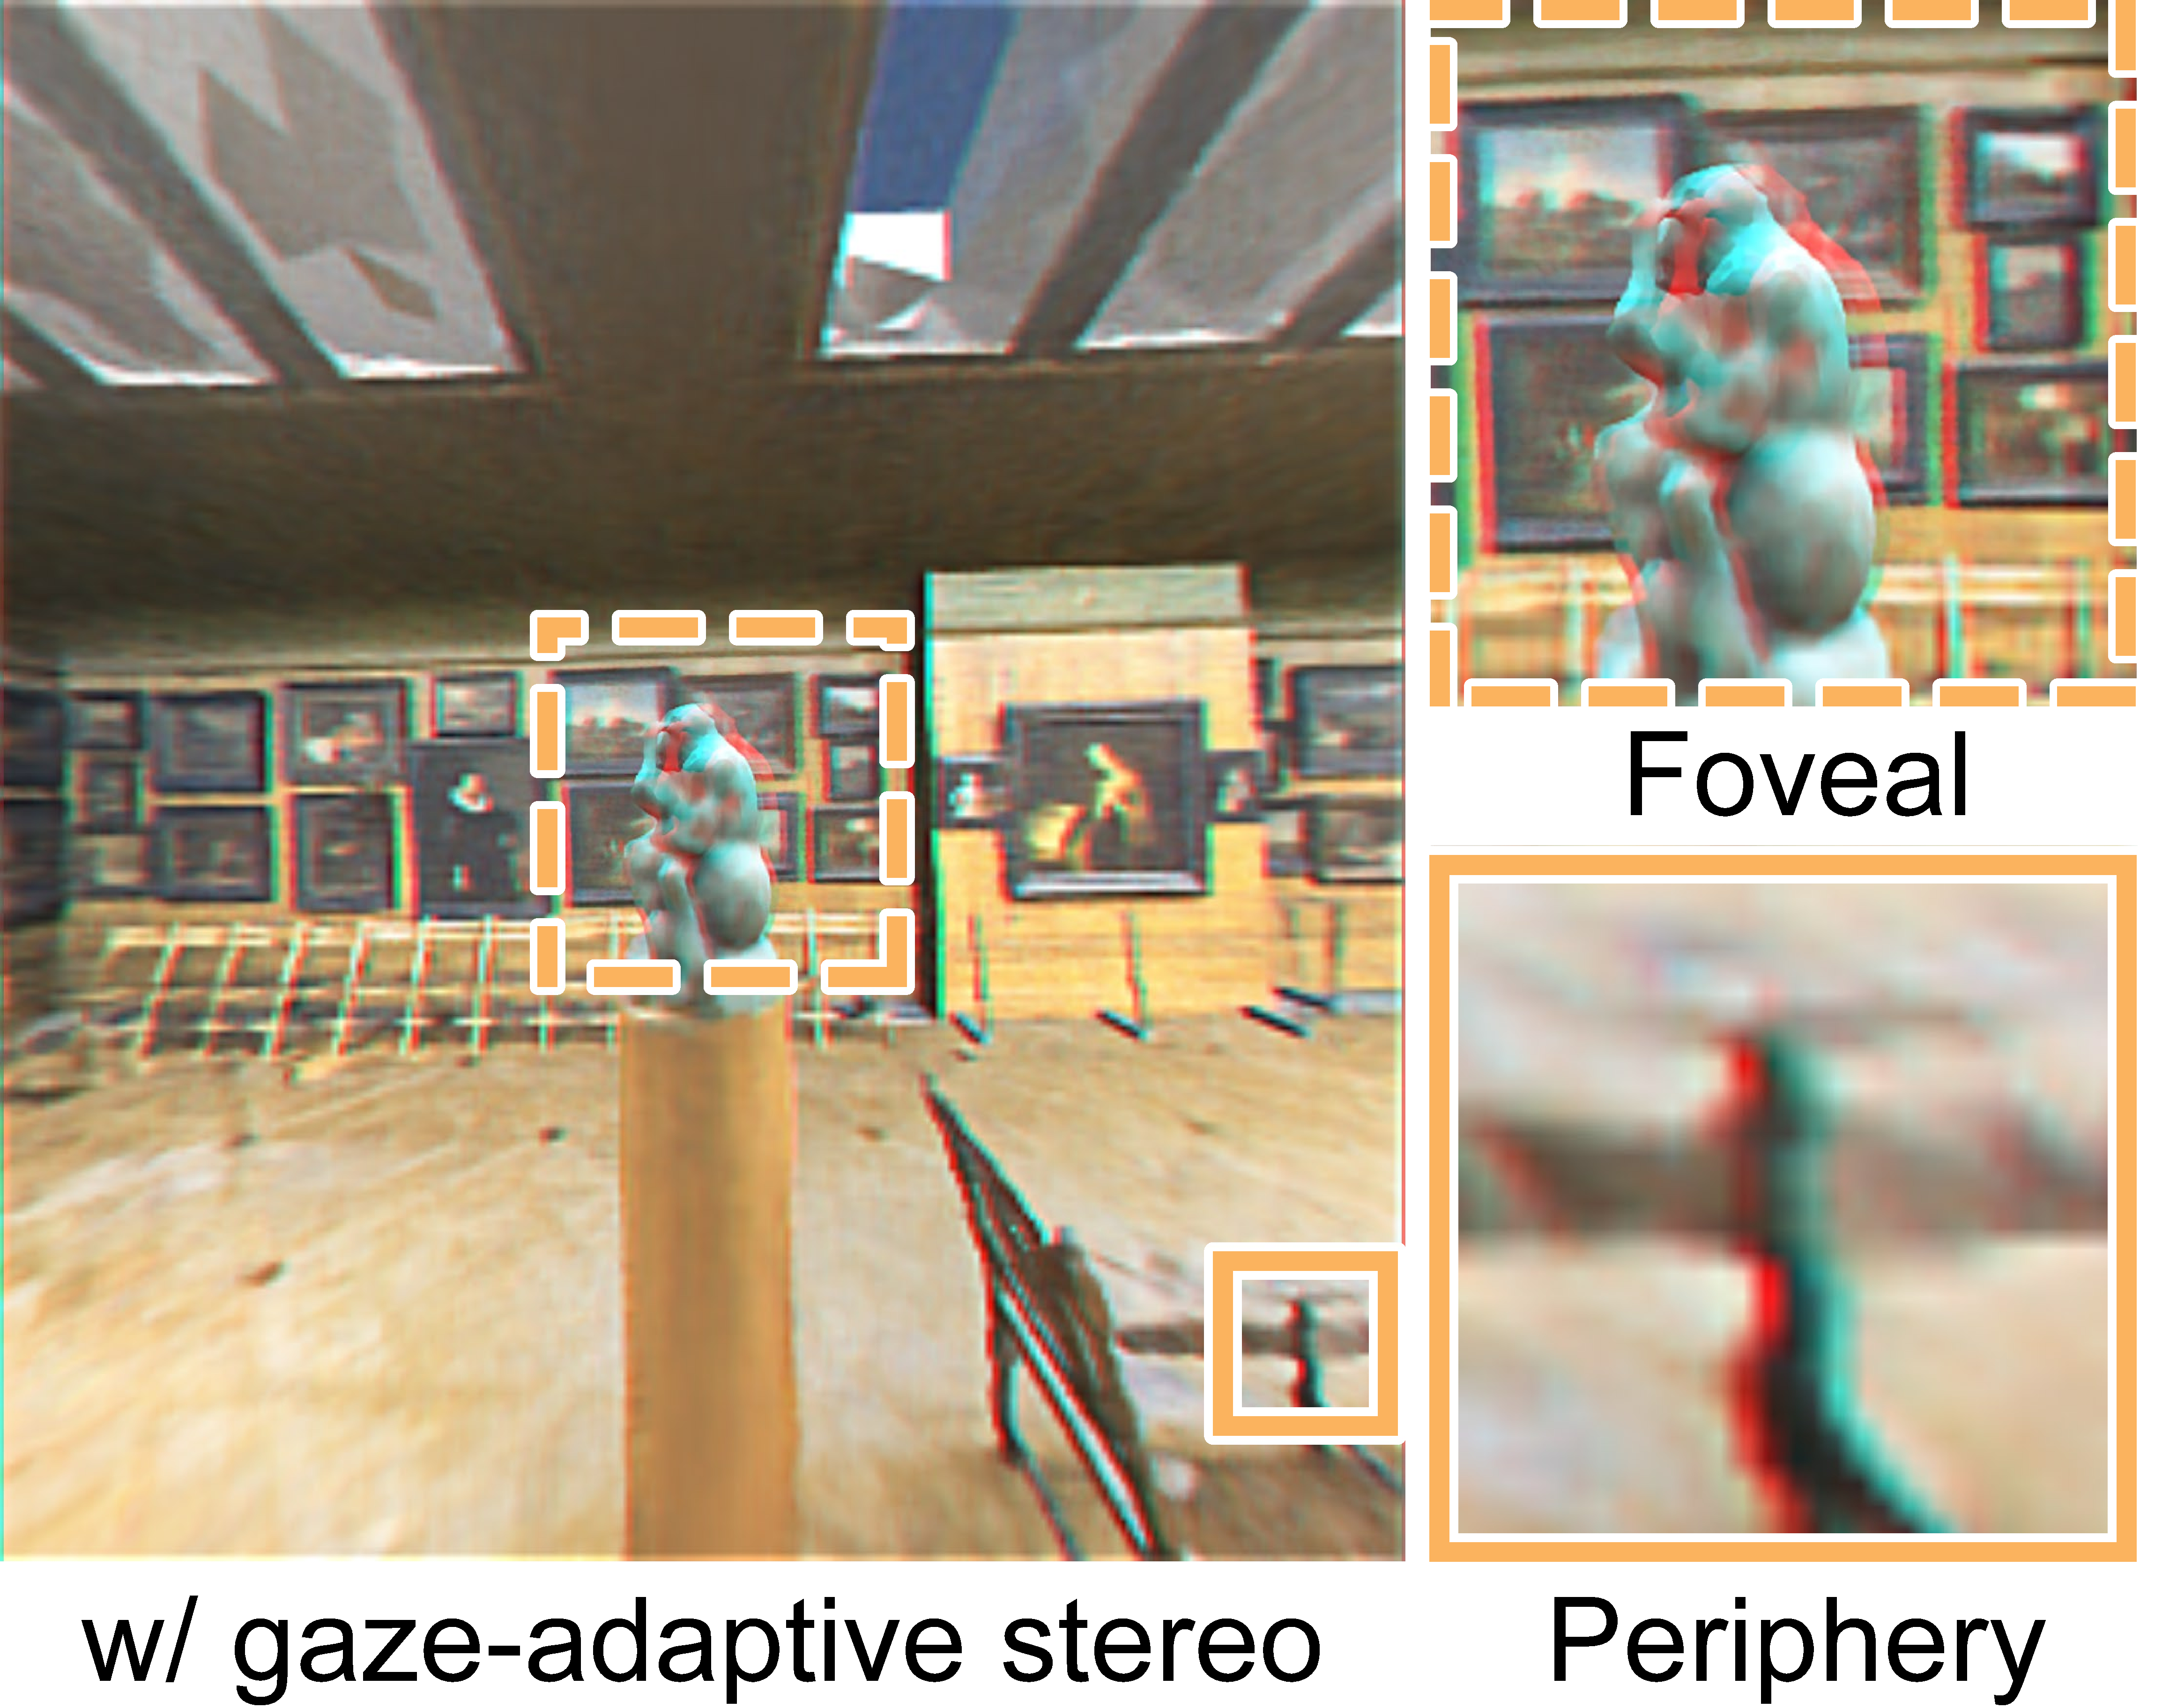
\includegraphics[width=0.48\linewidth]{TOG/figs/stereo_periphery/mono_periphery.pdf}\label{fig:mono:w}}
    %\subfloat[w/o gaze-adaptive stereo]{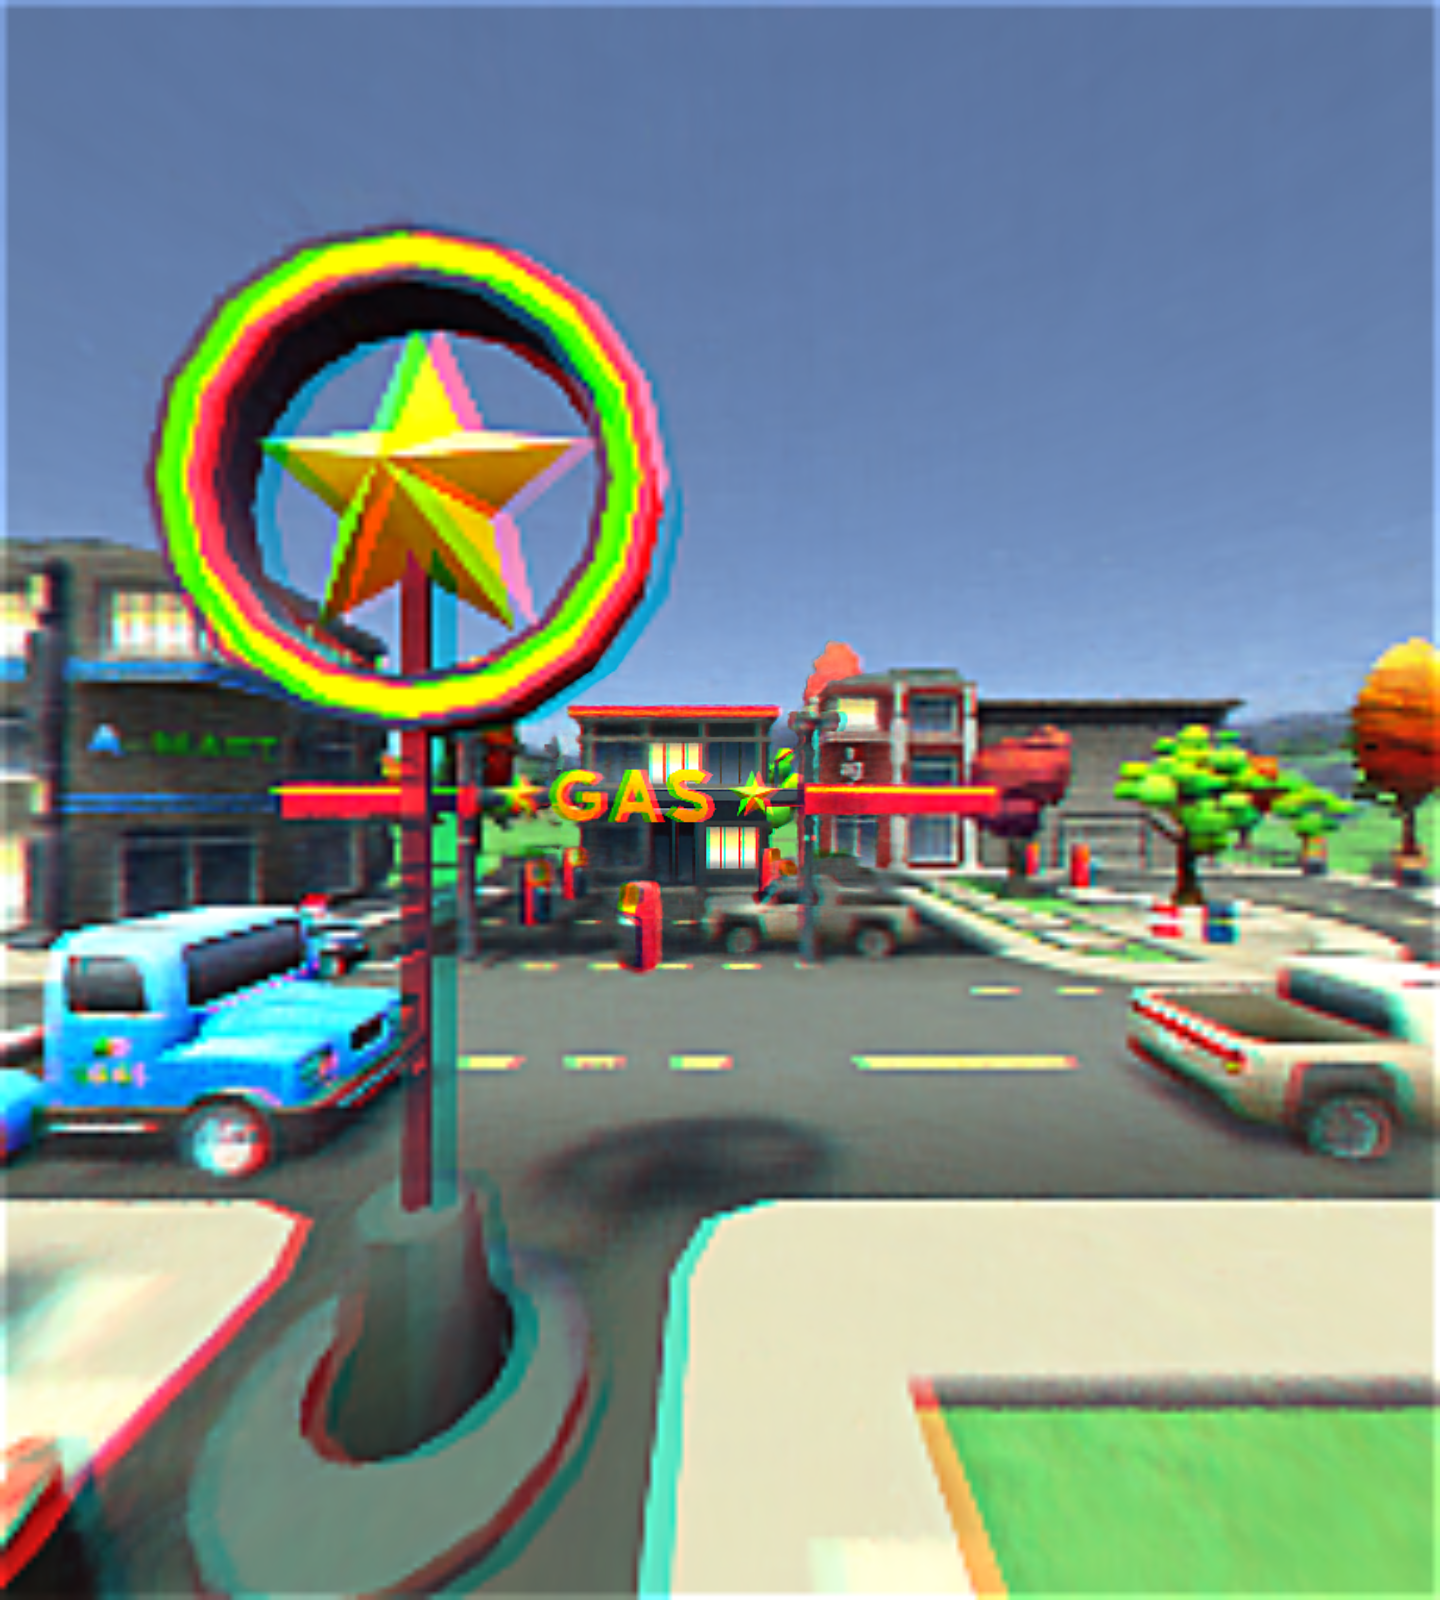
\includegraphics[width=0.248\linewidth]{TOG/figs/stereo_periphery/gas_view0000_blended_stereo.png}\label{fig:mono:wo}}
    %\subfloat[w/ gaze-adaptive stereo]{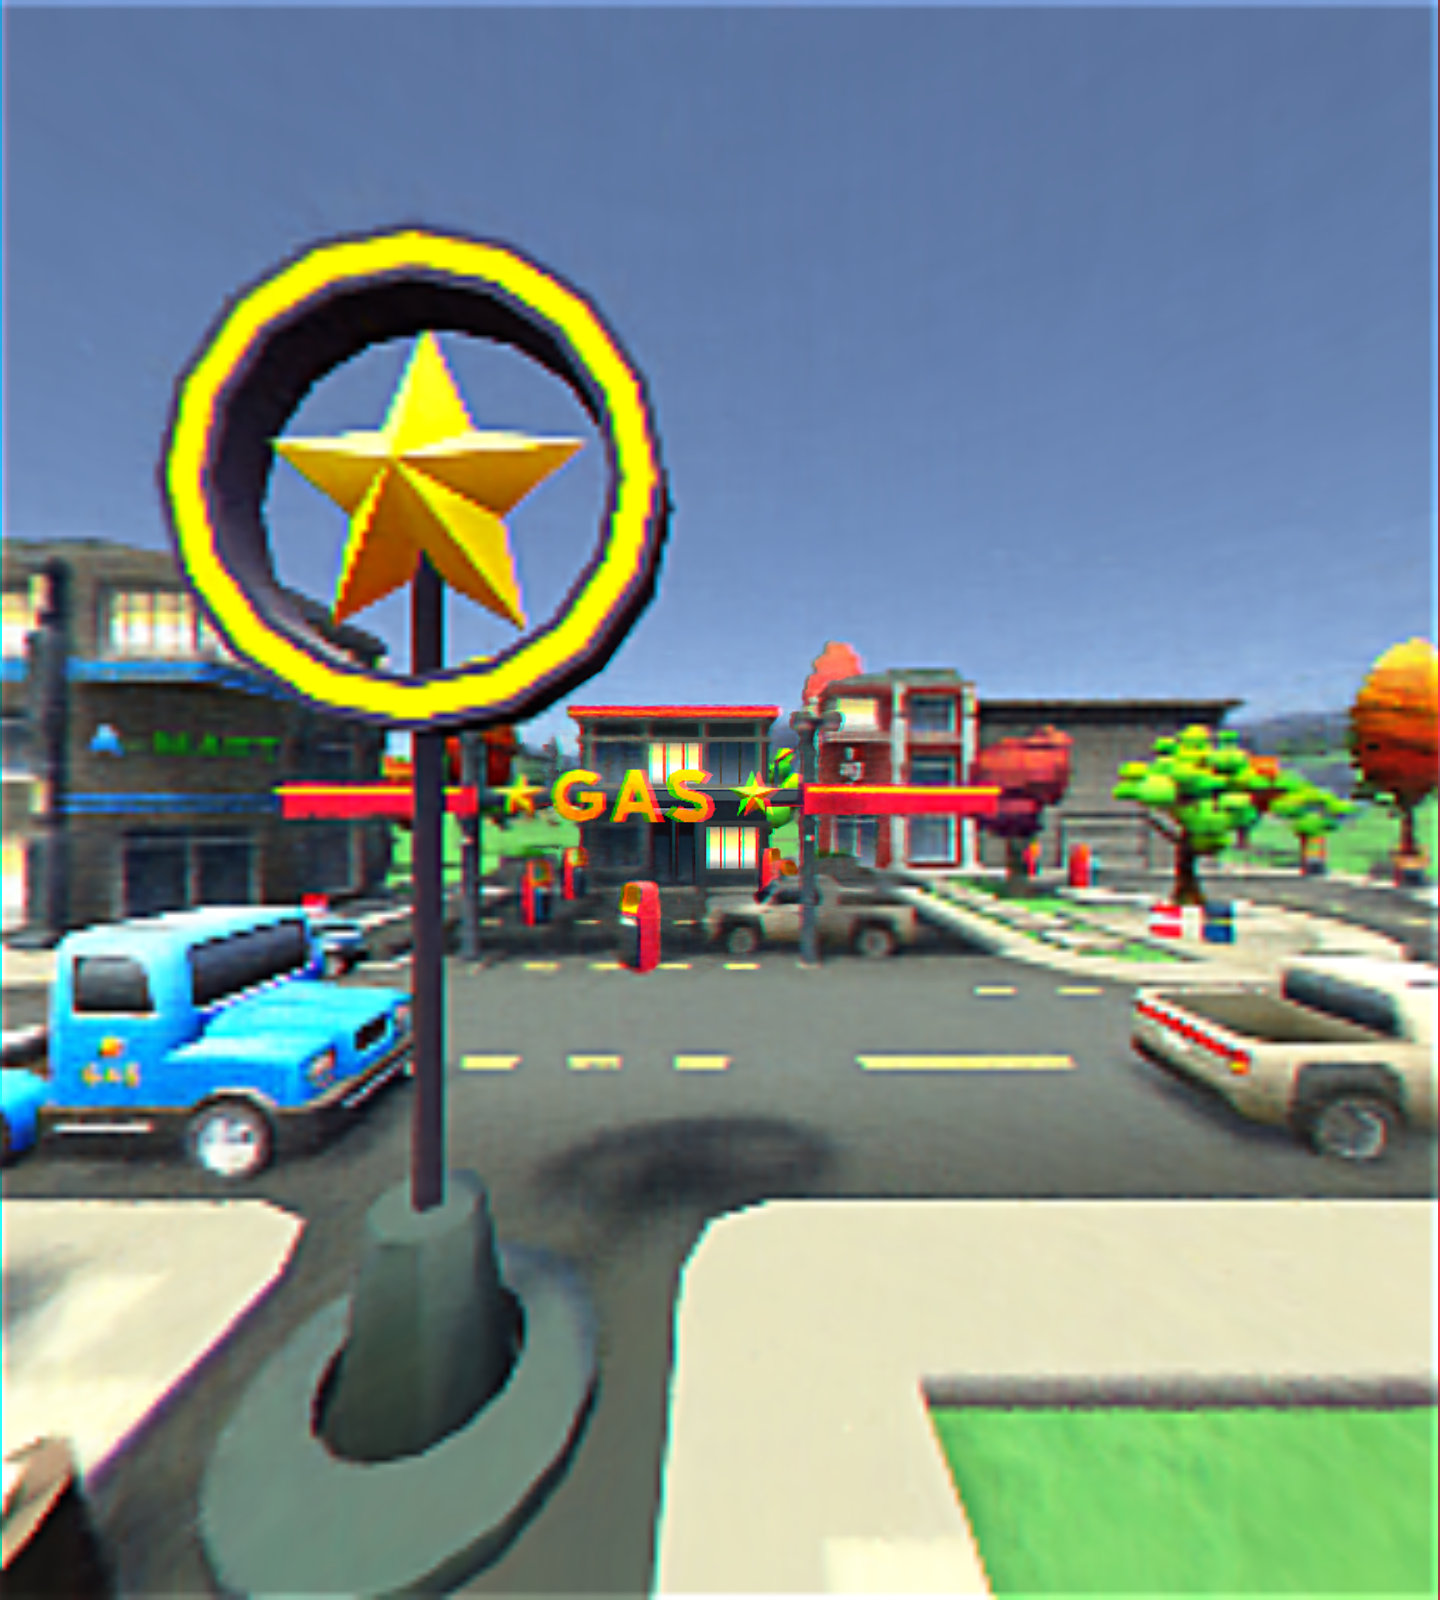
\includegraphics[width=0.248\linewidth]{TOG/figs/mono_periphery/gas_view0000_blended_stereo.png}\label{fig:mono:w}}
    
    %\subfloat[w/o gaze-adaptive stereo]{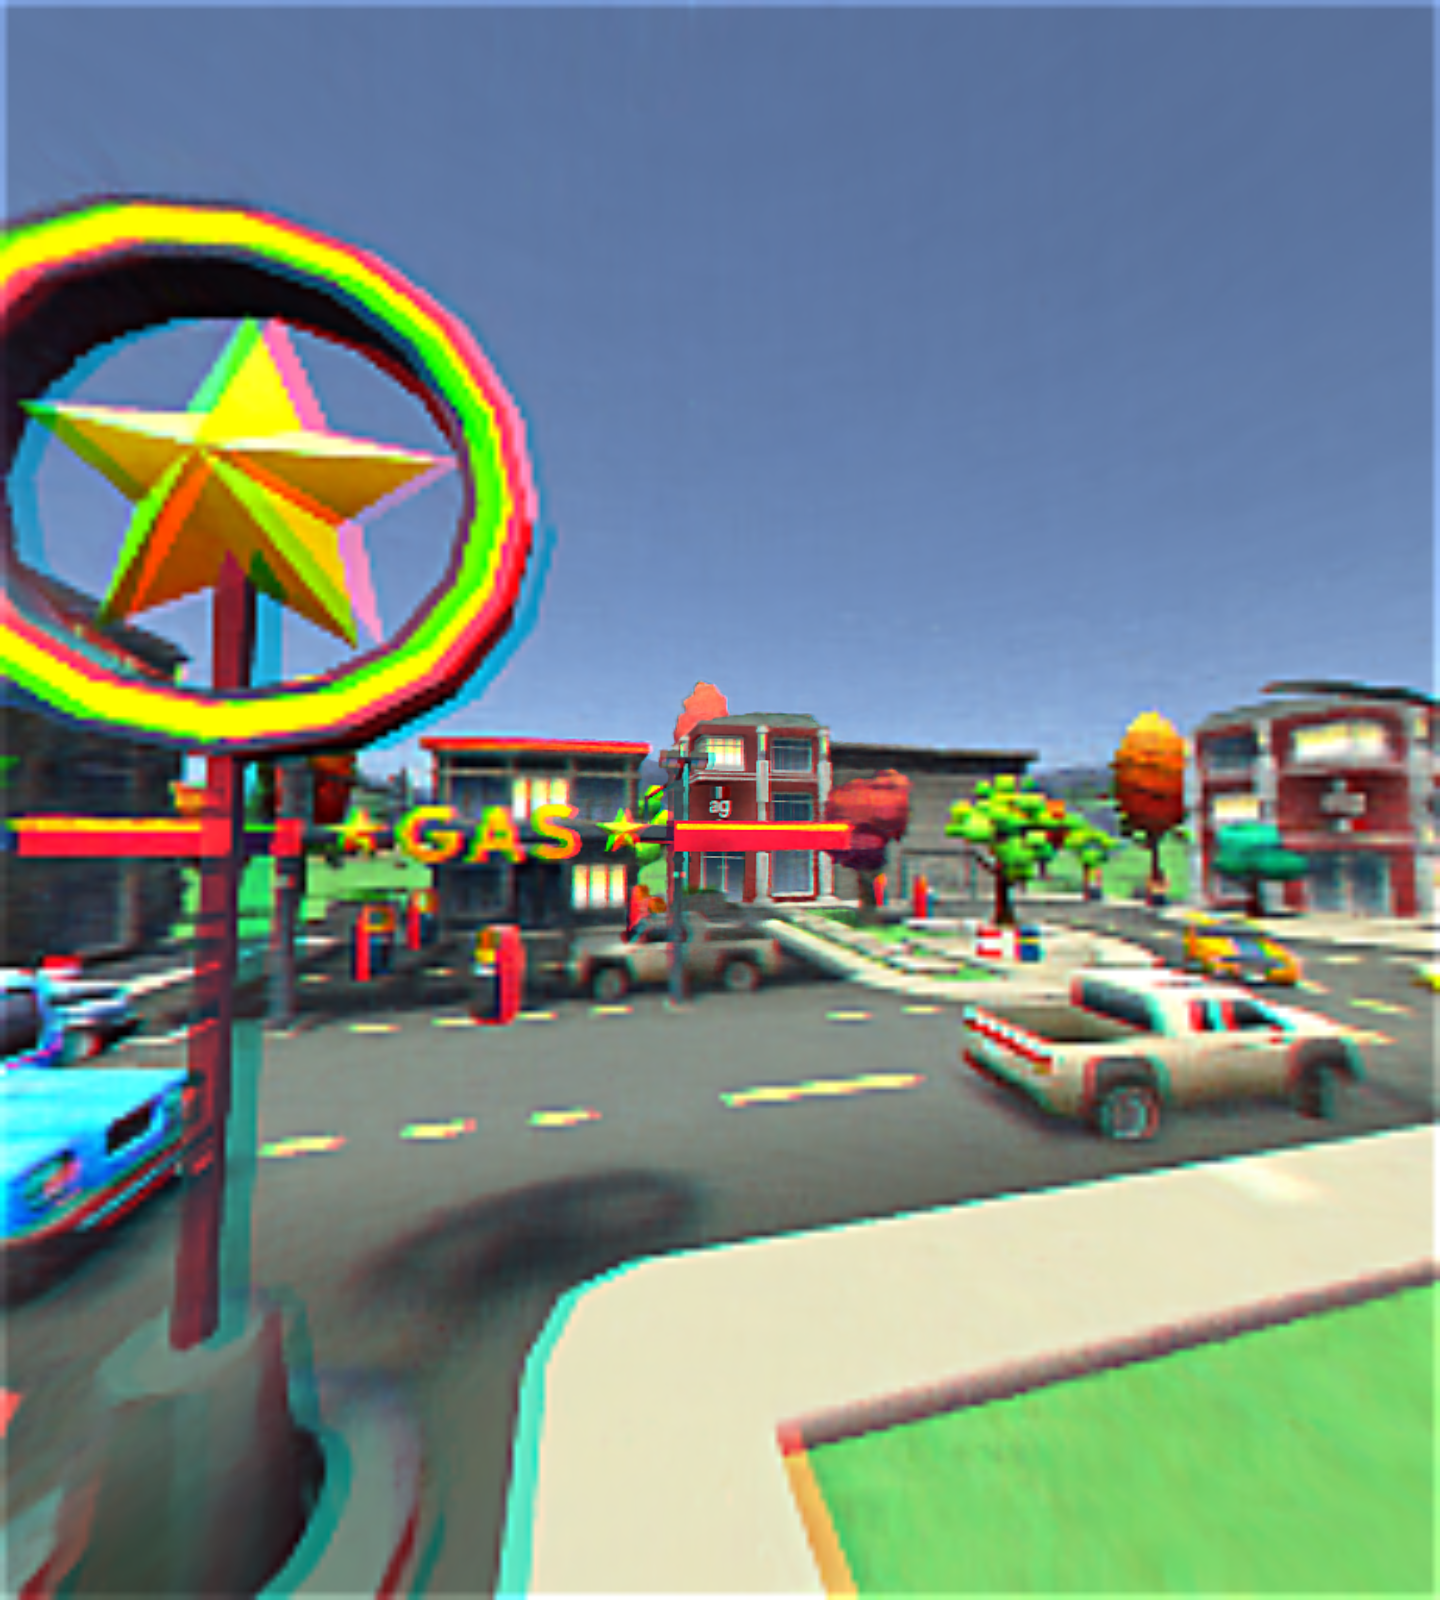
\includegraphics[width=0.248\linewidth]{TOG/figs/stereo_periphery/gas_view0001_blended_stereo.png}\label{fig:mono:wo}}
    %\subfloat[w/ gaze-adaptive stereo]{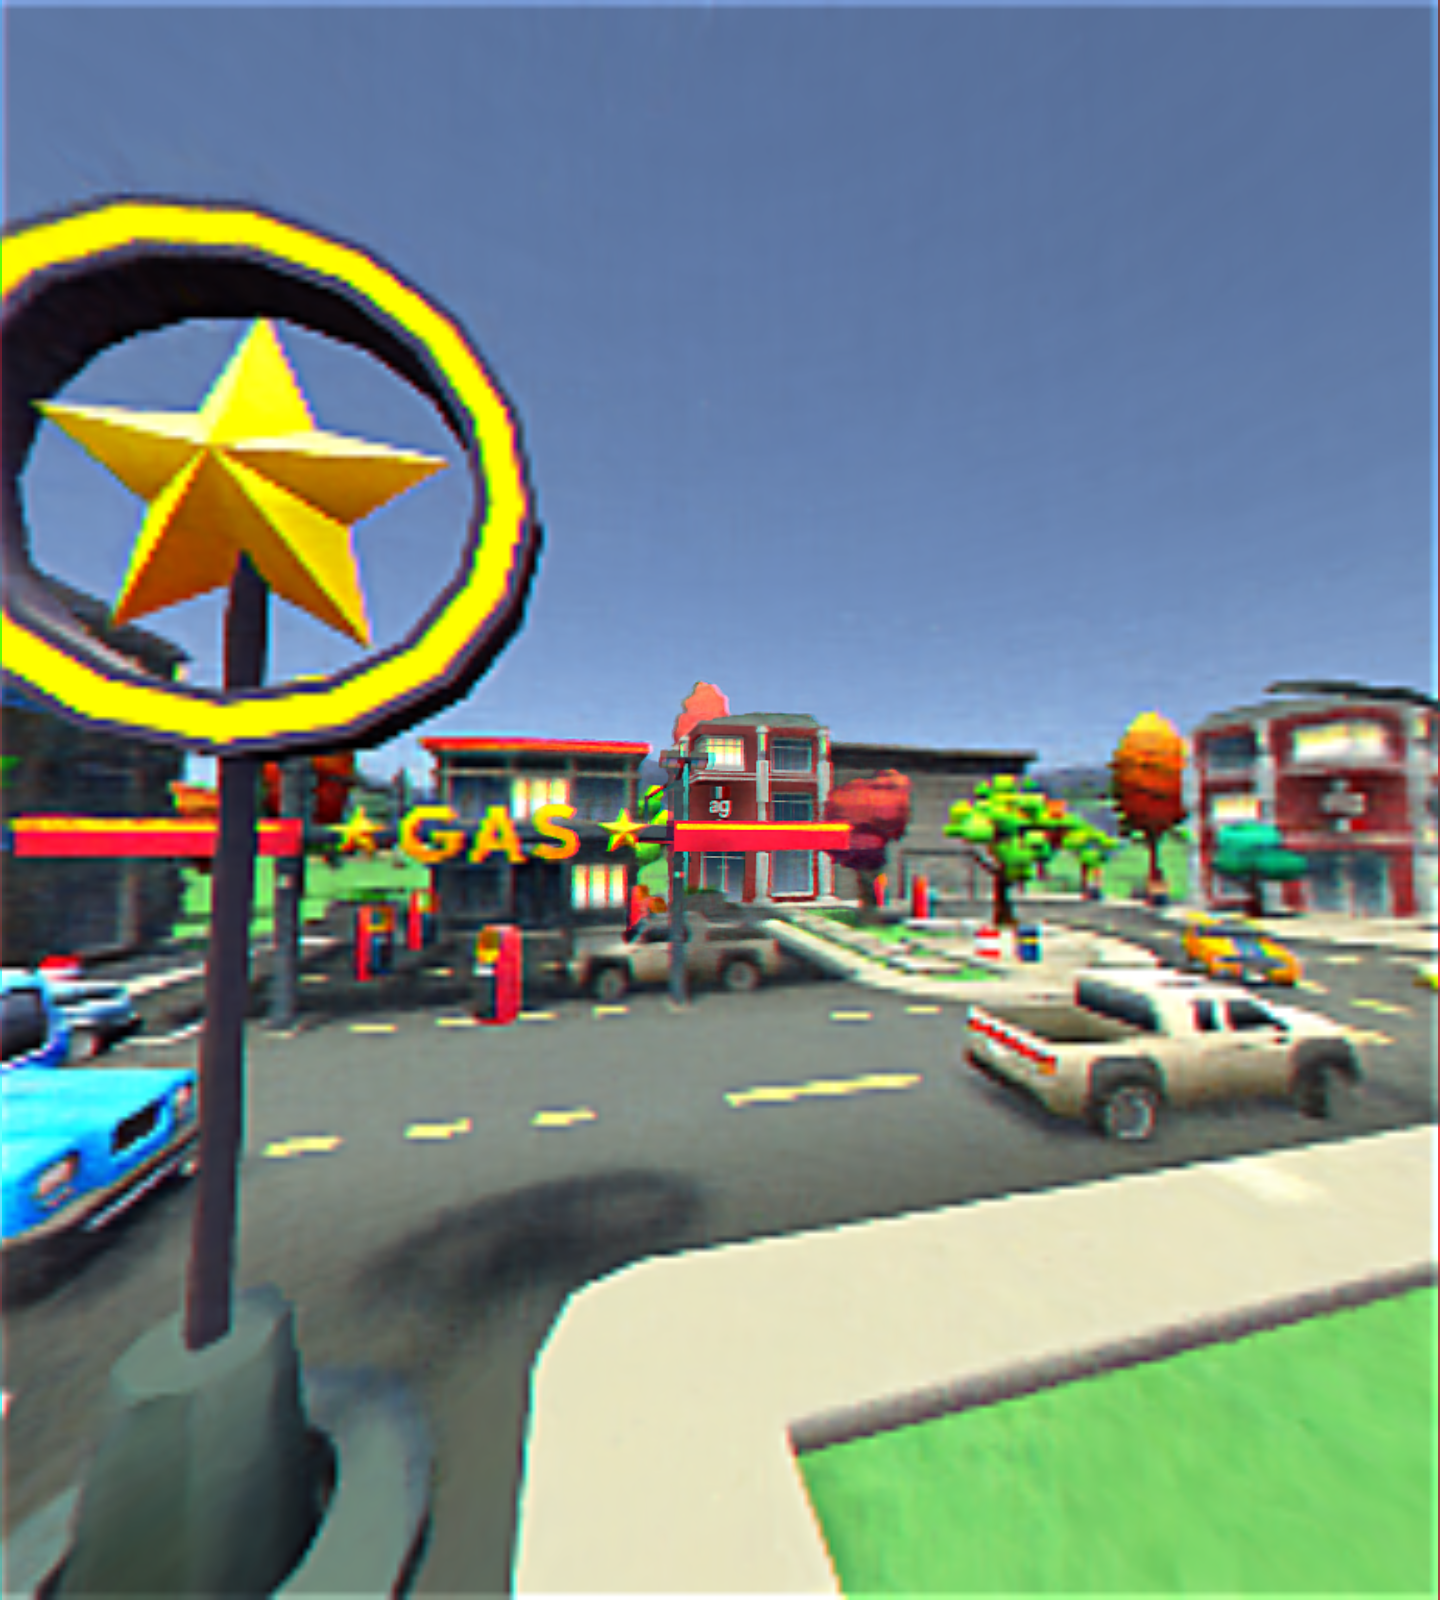
\includegraphics[width=0.248\linewidth]{TOG/figs/mono_periphery/gas_view0001_blended_stereo.png}\label{fig:mono:w}}
    \Caption{Visualization of the adaptive stereo-acuity with anaglyph.}
    {%
    \subref{fig:mono:wo} shows the rendered image with 6 retinal sub-images ($\imageFoveal^{\{l,r\}}$, $\imageMid^{\{l,r\}}$, and $\imageFar^{\{l,r\}}$).
    \subref{fig:mono:w} shows the rendered image with our adaptive and accelerated inference considering foveated stereoacuity ($\imageFoveal^{\{l,r\}}$, $\imageMid^{\{c\}}$, and $\imageFar^{\{c\}}$). Our method preserves full stereopsis in the fovea while reducing the angular resolution in the periphery for accelerated inference.
    }
    \label{fig:mono}
\end{figure}
\subsubsection{Real-time frame composition}%\dnc{May be moved to section 4 (merge with the paragraph 'Integration'). I think it's not closely related to our methodology and we have no key contributions about that. It's more like an engineering issue}\qisun{This whole section? I was concerned that would break the method completeness. Intentionally kept it short according to contribution level here.}
%\label{sec:method:blending}
%The individual elemental images are further blended as a single frame via a real-time image-based rendering. 
\begin{figure*}[ht]
    \centering
    \subfloat[network overlay]{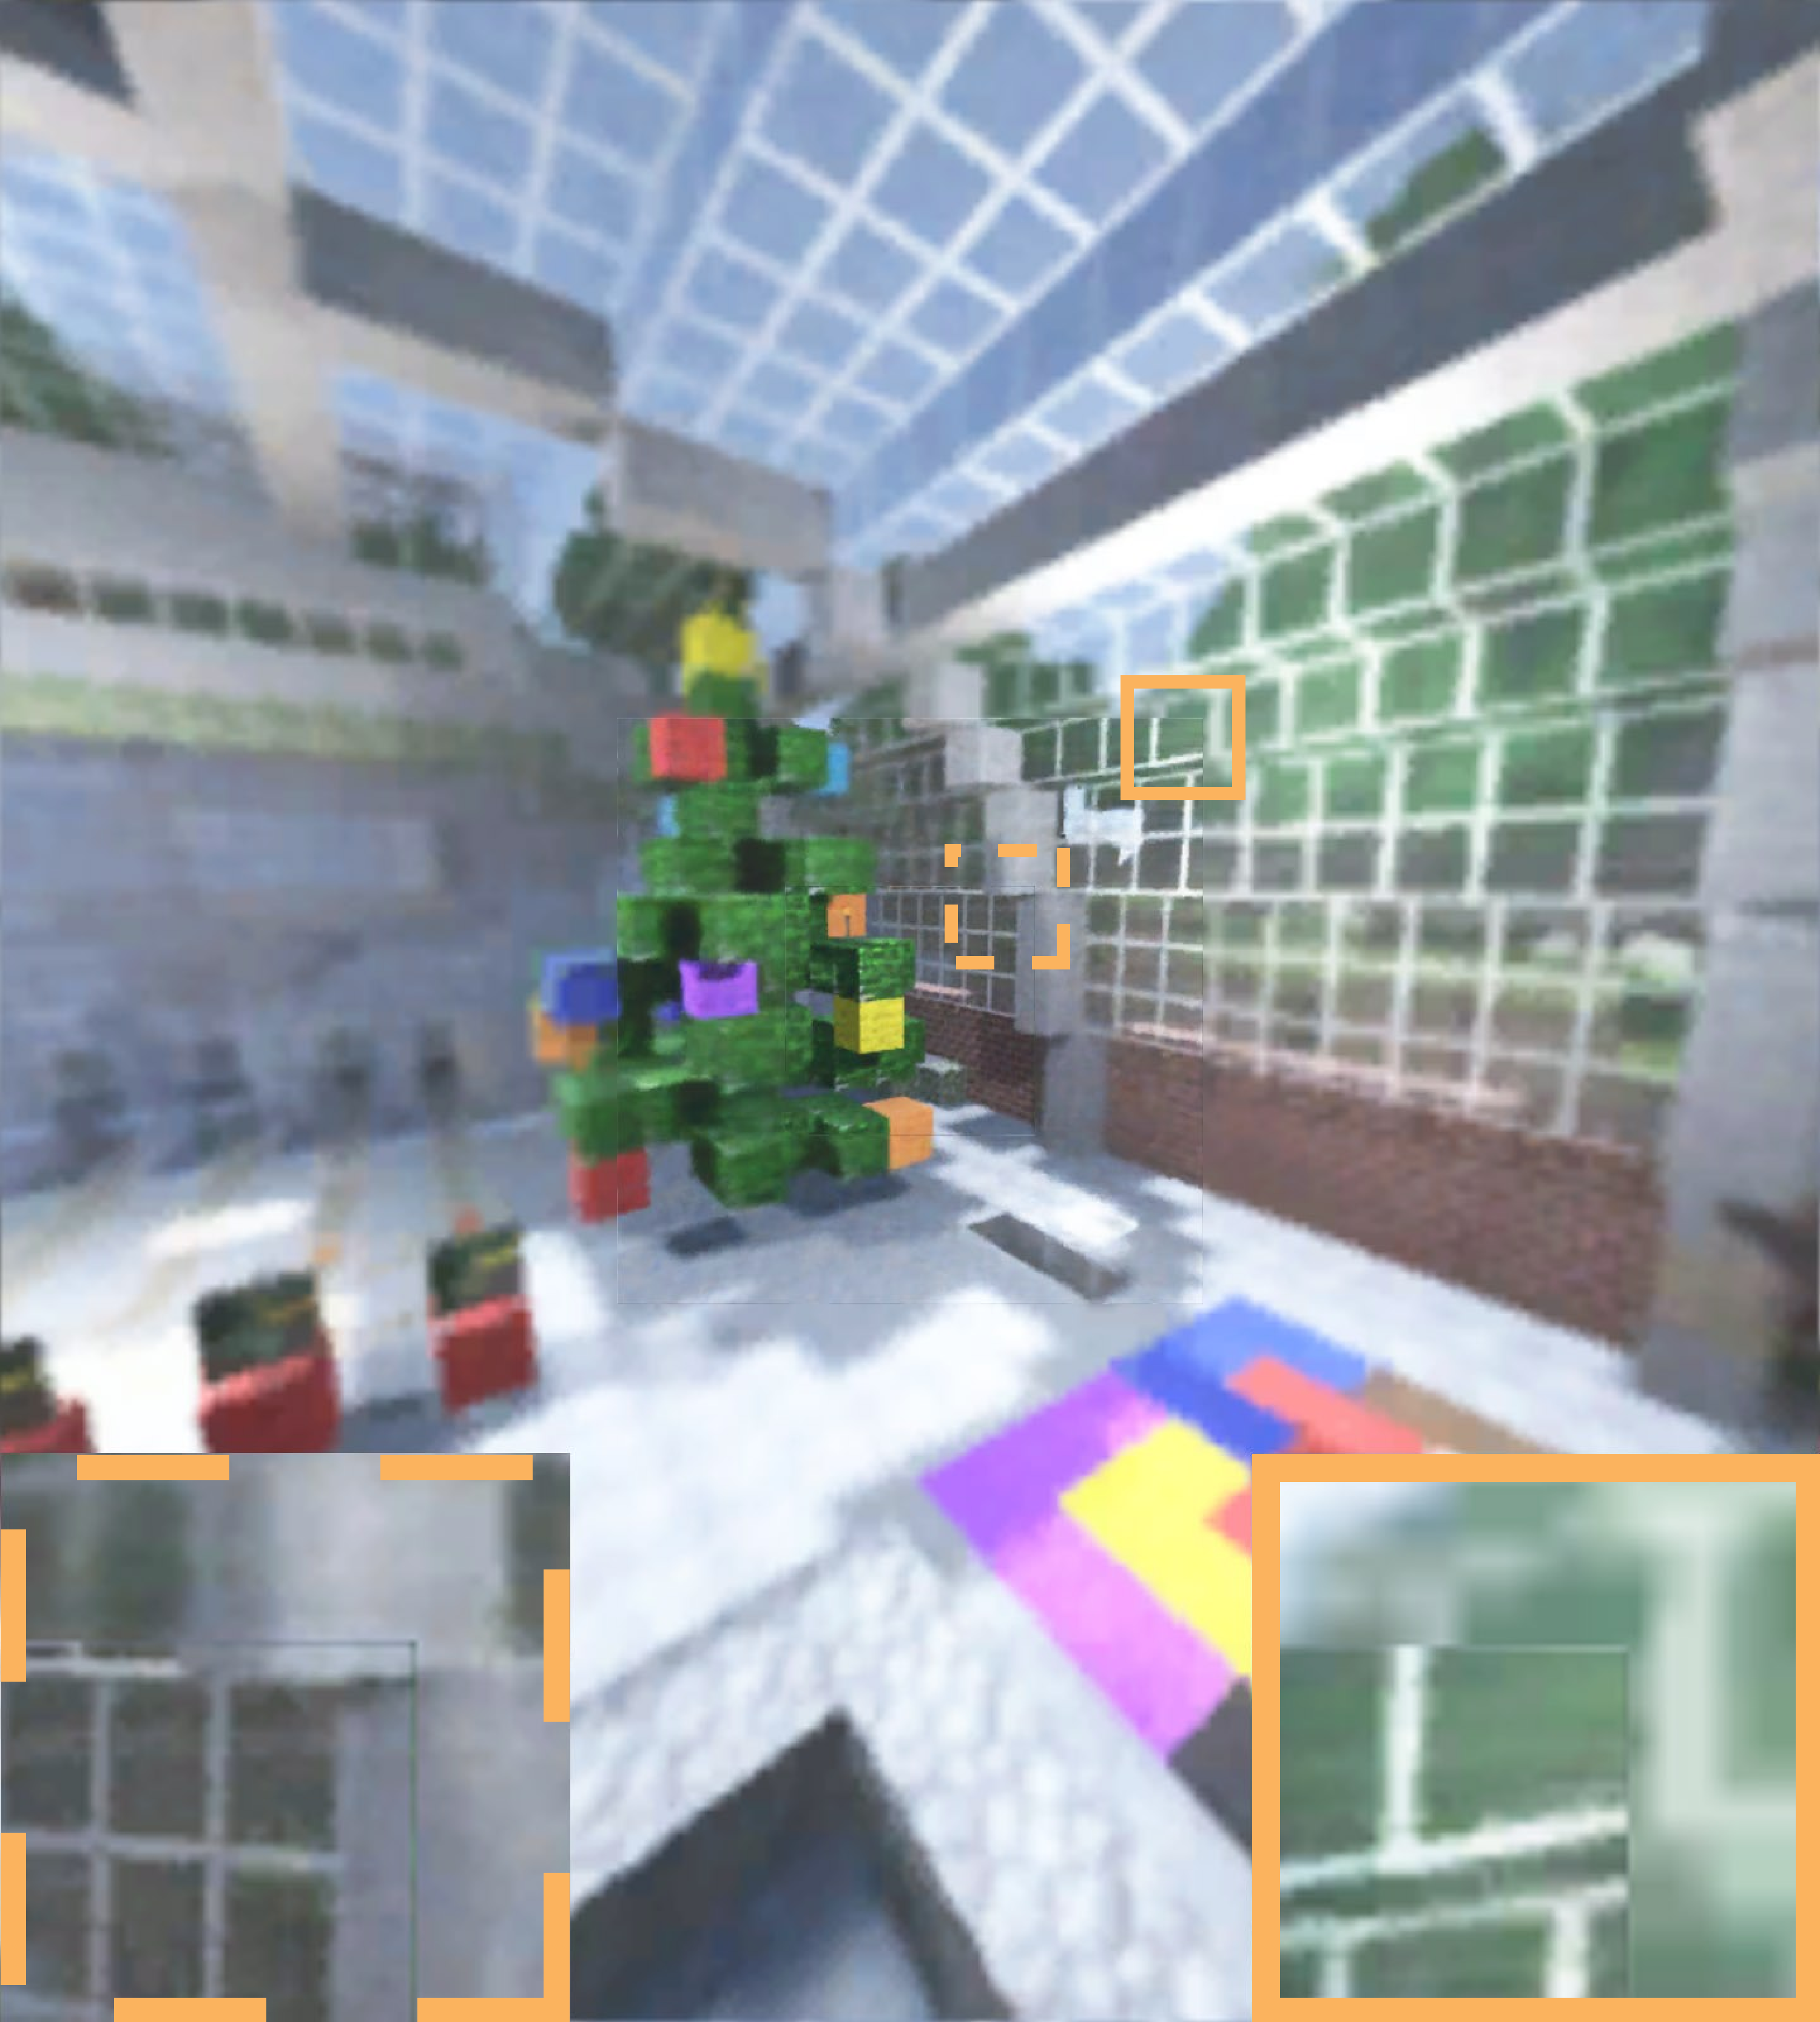
\includegraphics[width = 0.3\linewidth]{TOG/figs/system/overlap2.pdf}\label{fig:method:blending:overlay}}\hspace{1em}
    \subfloat[blending]{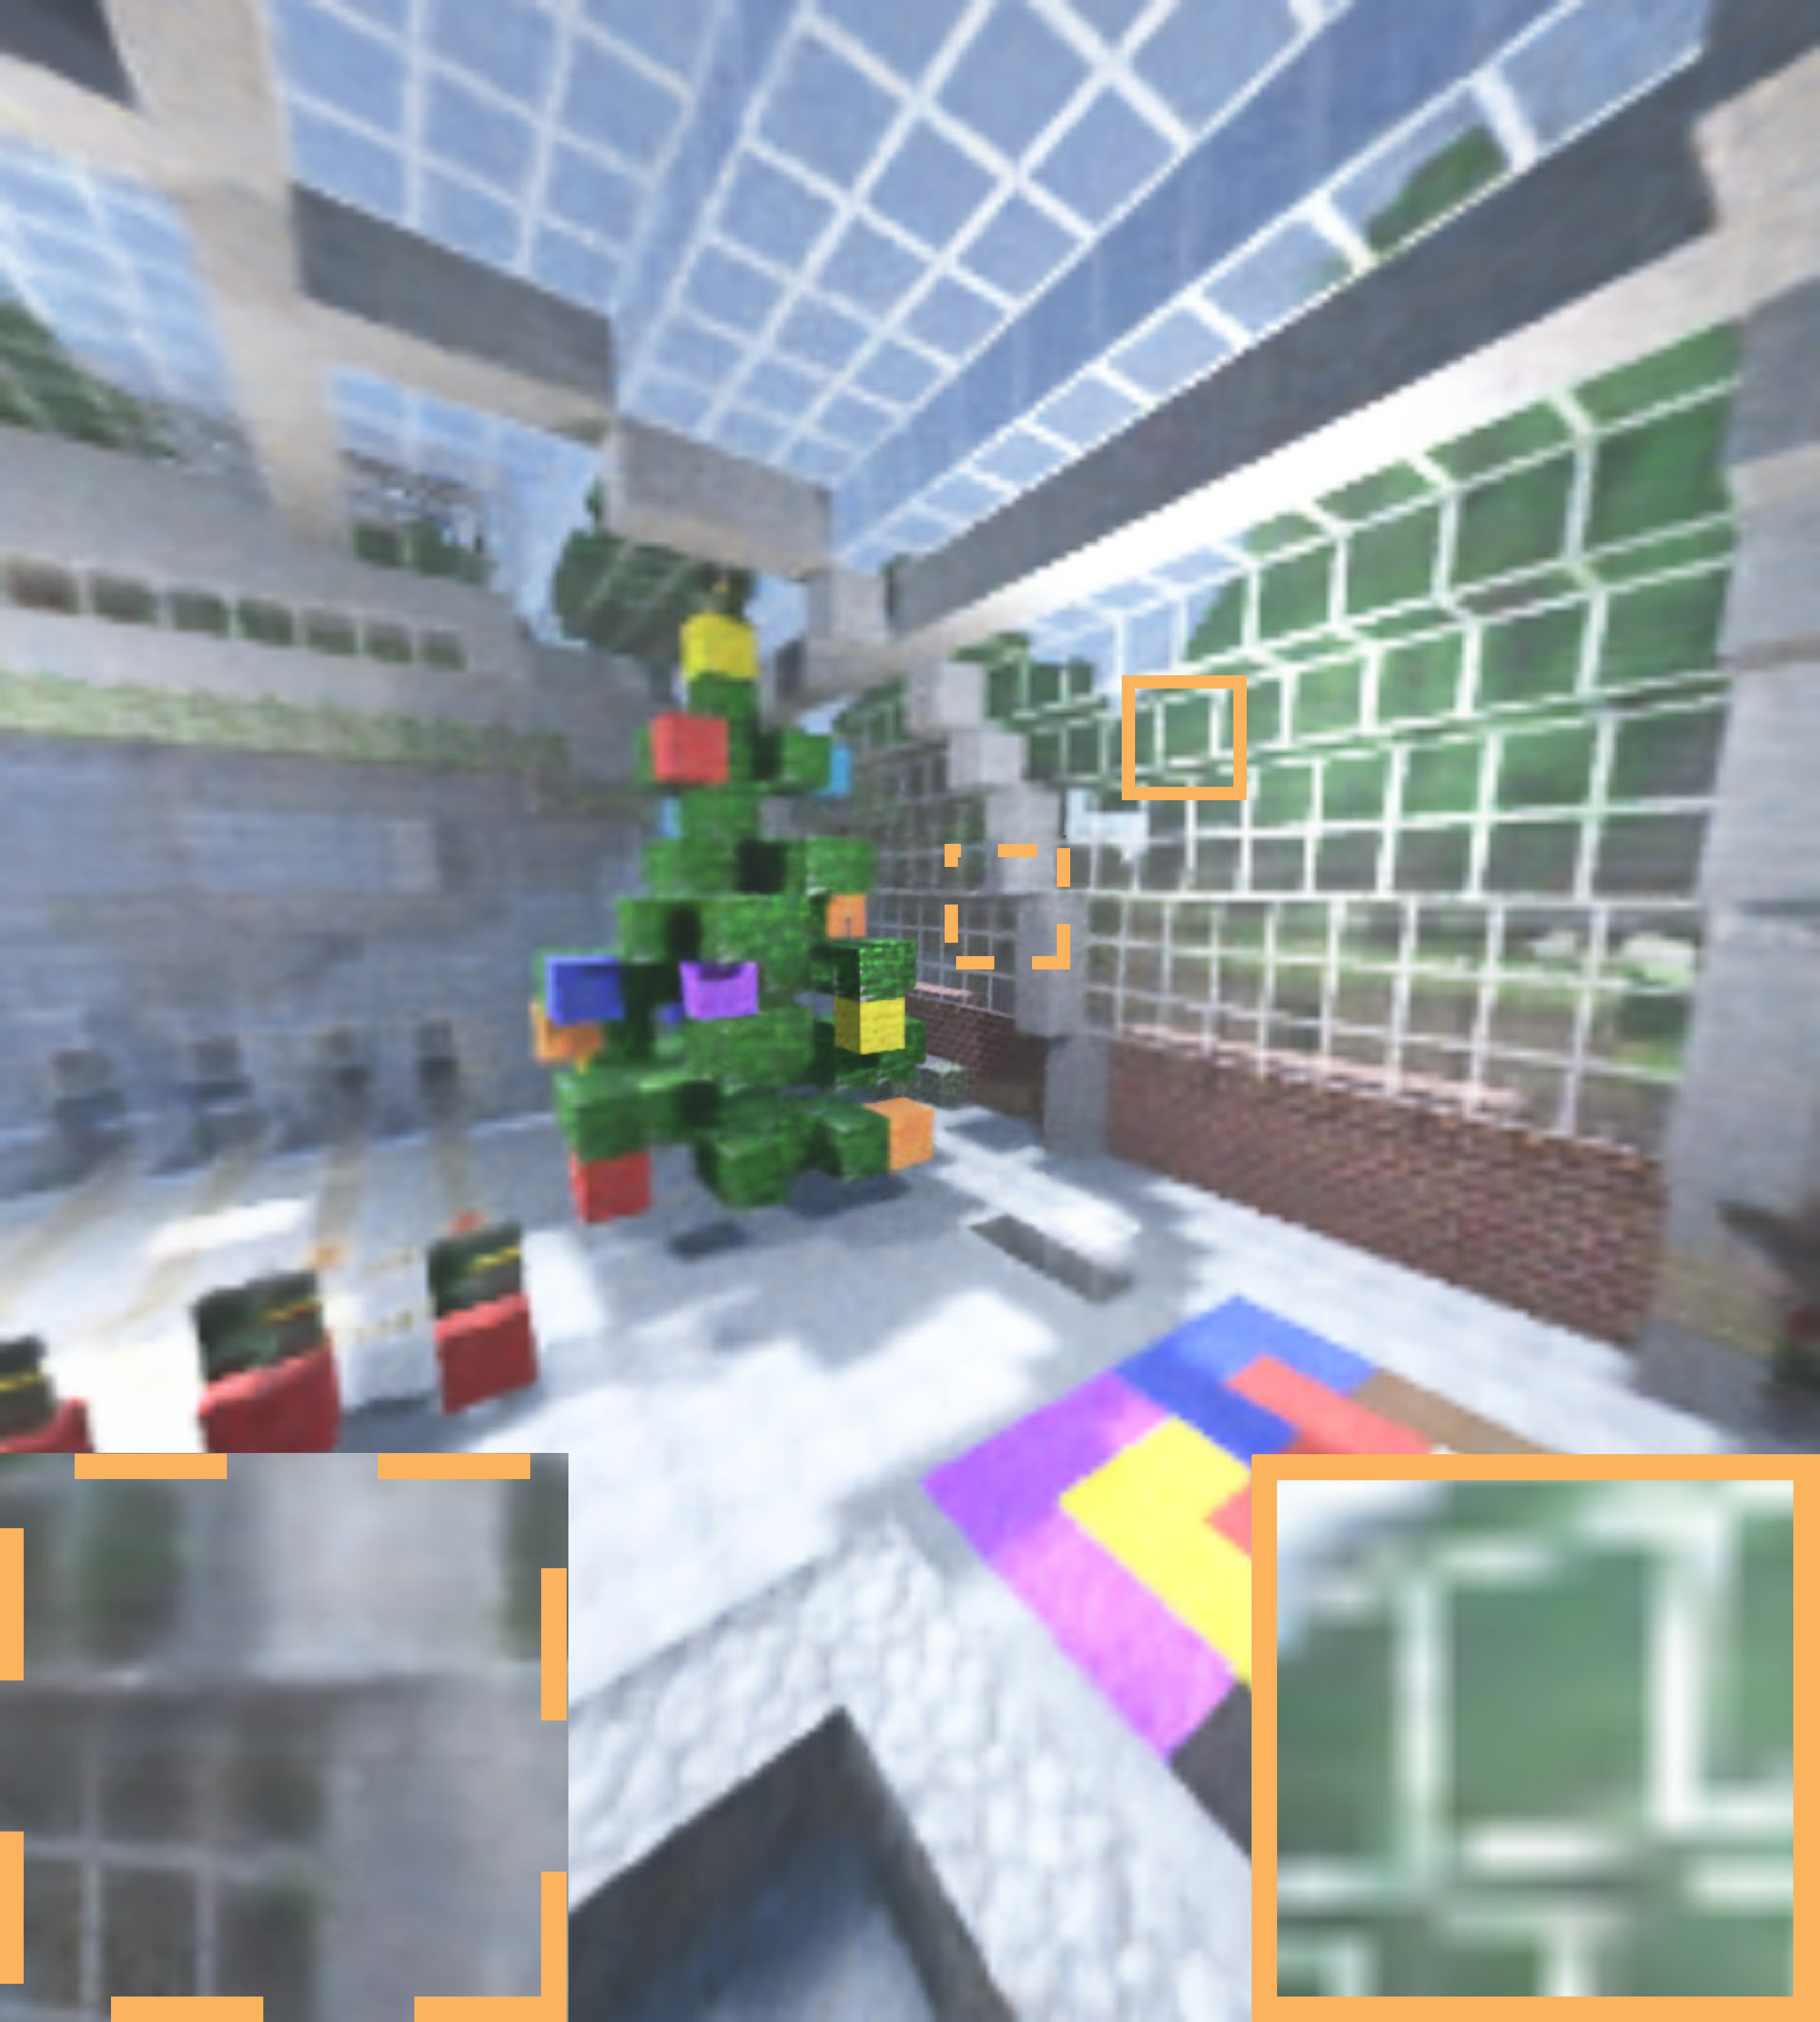
\includegraphics[width = 0.3\linewidth]{TOG/figs/system/blended2.pdf}\label{fig:method:blending:blending}}\hspace{1em}
    \subfloat[contrast enhancement]{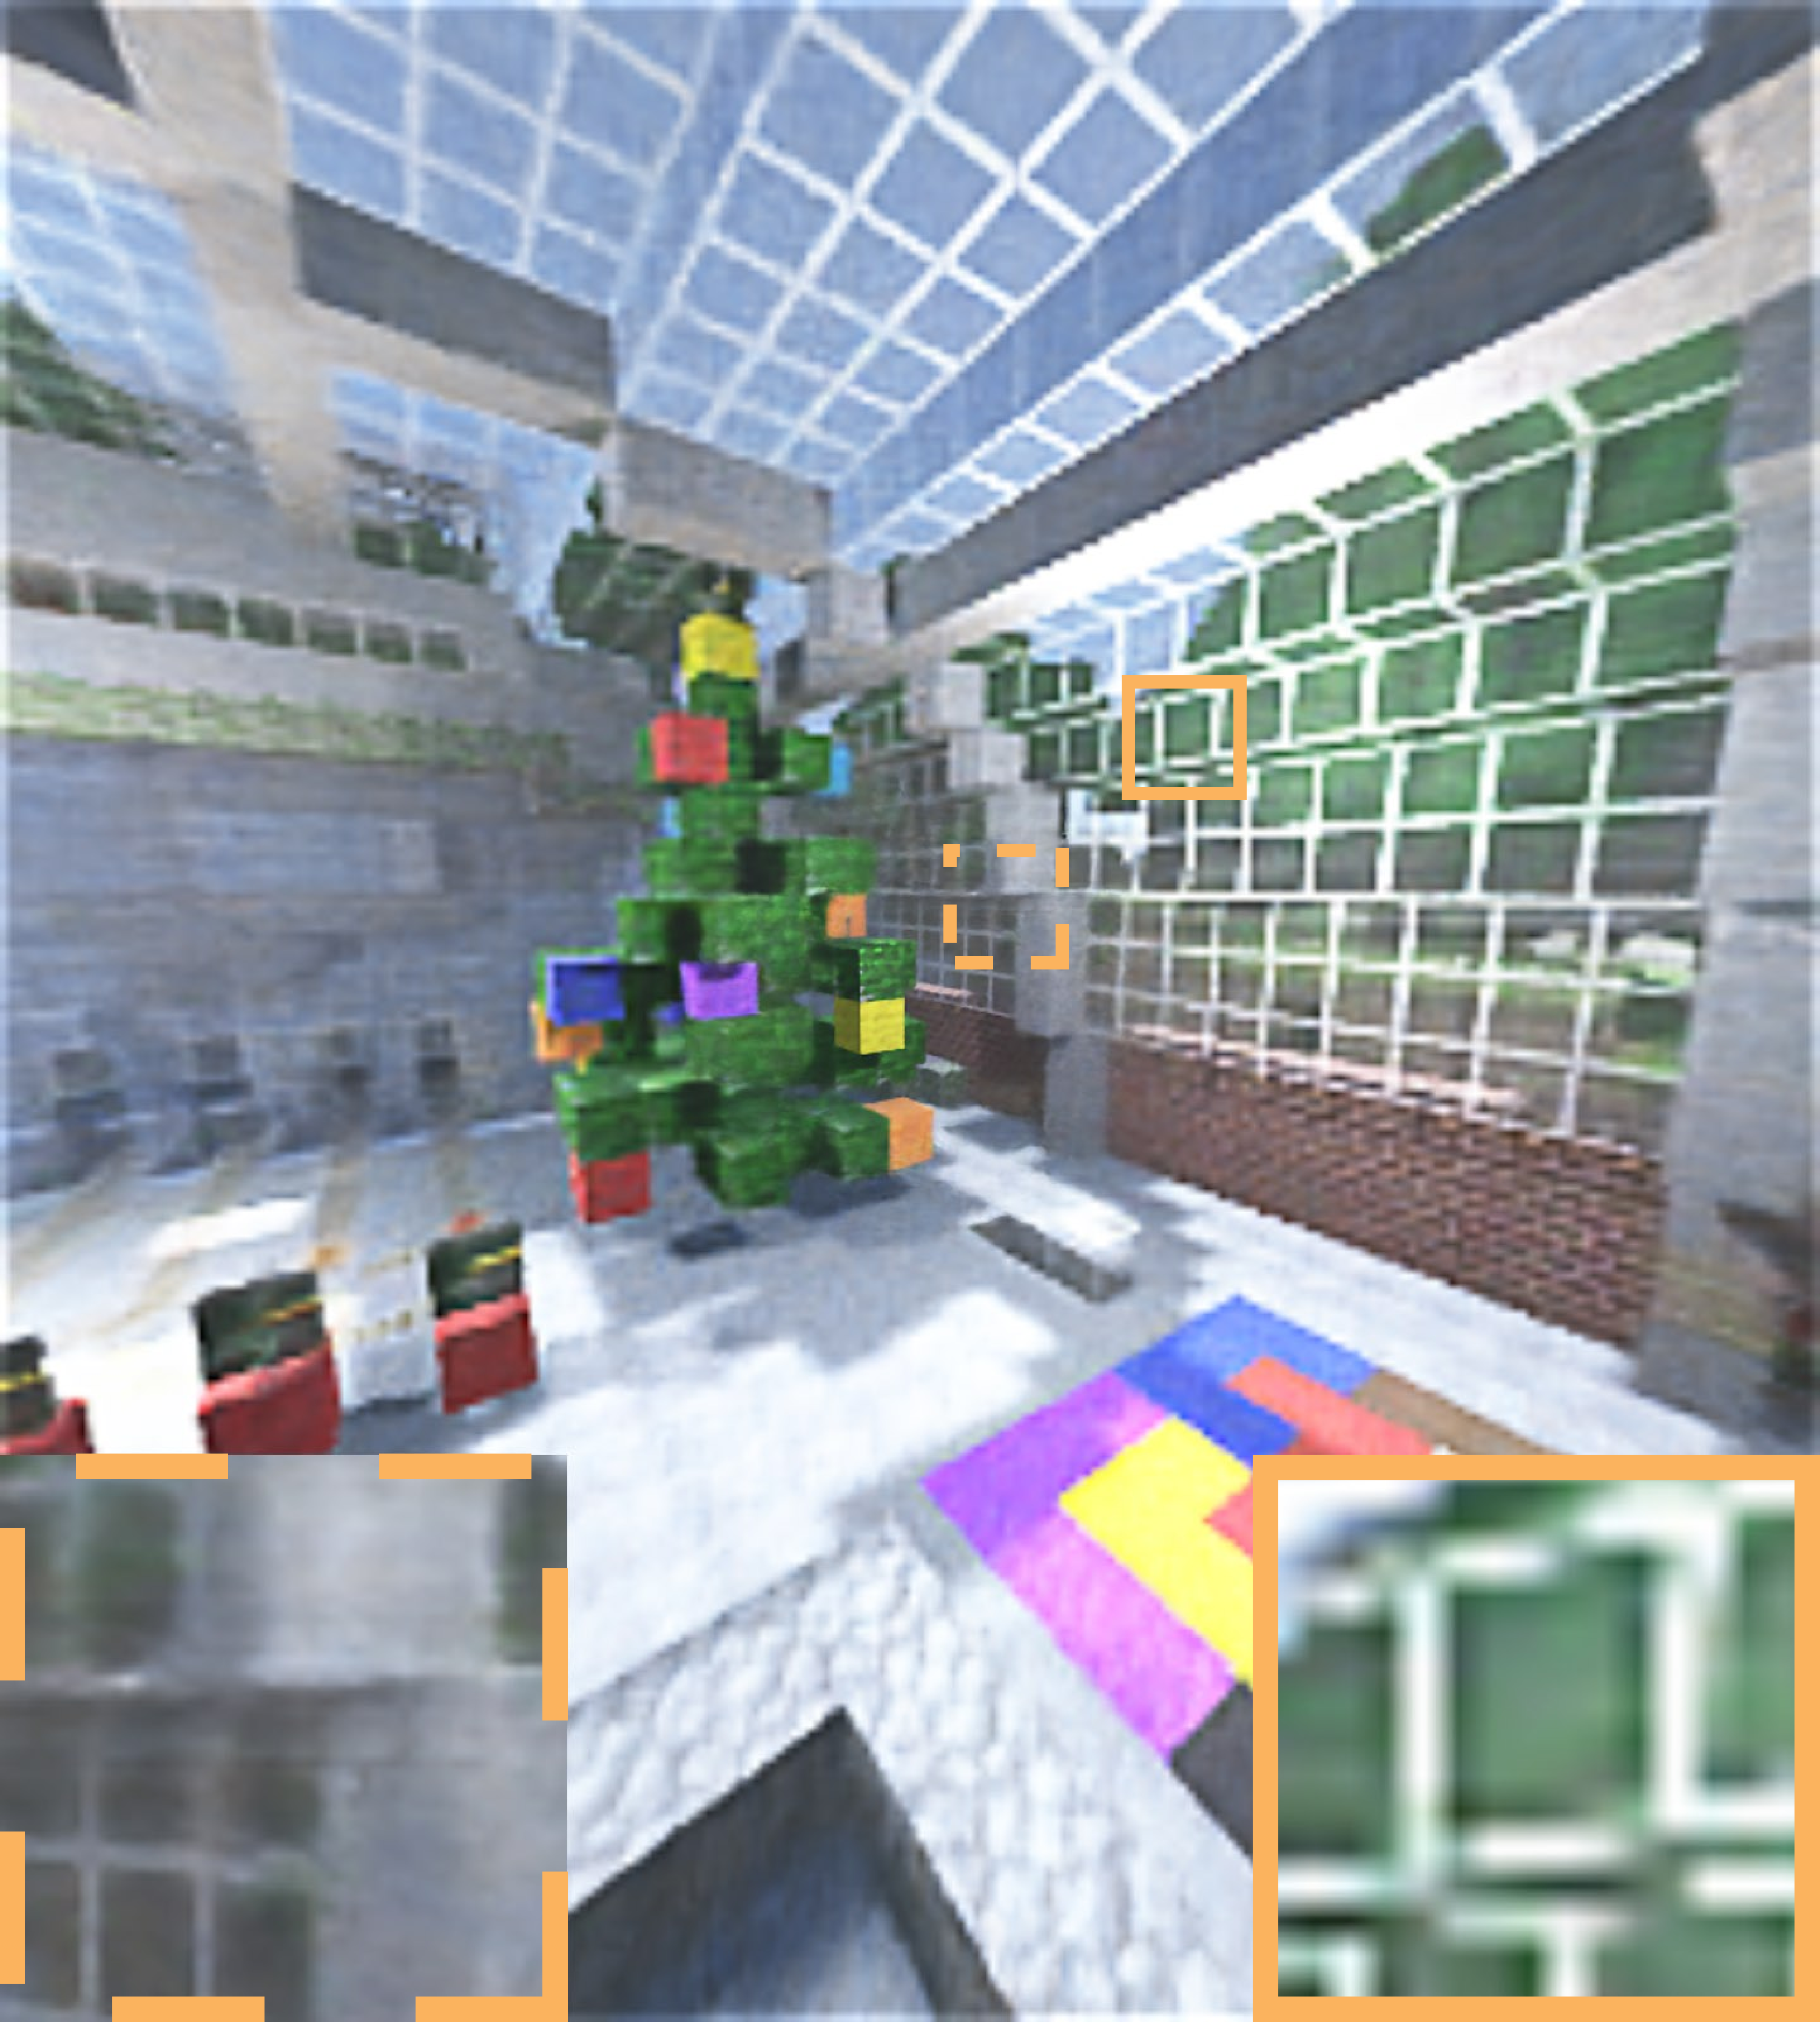
\includegraphics[width = 0.3\linewidth]{TOG/figs/system/blended_enhanced2.pdf}\label{fig:method:blending:contrast}}
    \Caption{Our multi-layer real-time rendering system.}
    {%
    \subref{fig:method:blending:overlay} shows the original 3-layer image output overlaid.
    \subref{fig:method:blending:blending} shows the result with cross-layer blending that enables smooth appearance on the edges.
    \subref{fig:method:blending:contrast} shows the contrast-enhanced rendering pass in the periphery.
    }
    \label{fig:method:blending}
\end{figure*}
With the obtained elemental images as input, an image-based rendering in the fragment shader is then executed to generate final frames for each eye (\Cref{fig:system:blending}).
%In real-time, we perform a image-based rendering that blends the elemental images. 
The output frames are displayed on the stereo VR HMDs.
{
Two adjunct layers are blended using a smooth-step function across $40\%$ of the inner layer.
This enhances visual consistency on the edges between layers \cite{Guenter:2012:F3G}.
}
To accommodate the mono-view $\imageMid^c$ and $\imageFar^c$, they are shifted towards each eye according to approximated foveal depth range.
%\nothing{we shift it with $-/+ \frac{\rayo^r-\rayo^l}{2}$ for left/right eye respectively. }
Lastly, we enhance the contrast following the mechanism of \cite{Patney:2016:TFR} to further preserve peripheral elemental images' visual fidelity due to its low PDD. The details are visualized in \Cref{fig:method:blending}. %\dnc{Note: the contrast enhancement is performed on elemental images, before blending. Different enhancement parameters are applied for fovea, mid and periph layers}

\subsection{Latency-Quality Joint Optimization}
\label{sec:method:optimization}
As a view synthesis system based on sparse egocentric representation (the $\sphereNum$ spheres) and neural networks (the $\mlpLayerNum, \mlpChannelNum$), the method inevitably introduces approximation errors. On the other hand, these variables also determine the online computational time that involves inferring function $\mlpFunc$ and ray marching the $\sphereNum$ spheres. 
However, VR strictly demands both quality and performance. We present a spatial-temporal model that analytically depicts the correlations and optimizes the variables for an ideal user experience.

\paragraph{Precision loss of a 3D scene}
As shown in \Cref{fig:notations}, under the egocentric representation, a 3D point $\pt$ is re-projected as the nearest point on a sphere that connects it to the origin point:
\begin{equation}\label{eq:closestPoint3D}
{\pt^\prime}(\sphereNum,\mathbf{\sphereRadius},\SpatialPt) \triangleq \sphereRadius_k \frac{\pt}{\norm{\pt}}, \ k=\argmin_{j\in[1,\sphereNum]}\left(\norm{\norm{\SpatialPt}-\sphereRadius_j}\right).
\end{equation}

Similar to volume-based representation, the multi-spherical system is also defined in the discrete domain. The sparsity thus naturally introduces approximation error that compromises the synthesis quality. To analytically model the precision loss, we investigate the geometric relationship among the camera, the scene, and the representation.
As illustrated in \Cref{fig:teaser:scene,fig:notations},  for a sphere (located at origin point) with radius $\sphereRadius$, its intersection (if exists) with a directional ray $\{\rayo,\rayd\}$ is
\begin{equation}
\intersectionFunc(\sphereRadius,\rayo,\rayd) = \rayo + \left({\left((\rayo\cdot\rayd)^2-\norm{\rayo}^2+\sphereRadius^2\right)}^{\frac{1}{2}}-\rayo\cdot\rayd\right)\rayd,
\label{eq:raySphereIntersection}
\end{equation}
where $\rayo$ and $\rayd$ are the ray's origin point and normalized direction, respectively.
% \begin{equation}
% \left\{\intersectionFunc(\sphereRadius_i,\rayo,\rayd) \right\}\ |\ i\in[1,2,\dots,\sphereNum].
% \end{equation}
Inversely, given a view point $\rayo$ observing a spatial location $\SpatialPt$, the ray connecting them has the direction $\rayd(\SpatialPt,\rayo)=\frac{\SpatialPt-\rayo}{\norm{\SpatialPt-\rayo}}$. This ray may intersect with more than one sphere. Among them, the closest one to $\SpatialPt$ is:
\begin{equation}\label{eq:closestPointImg}
\begin{aligned}
    \hat{\pt}&(\rayo,\sphereNum, \mathbf{\sphereRadius},\SpatialPt) \triangleq \\
    &\intersectionFunc(\sphereRadius_k,\rayo,\rayd(\SpatialPt,\rayo))\ |\ k=\argmin_{j\in[1,\sphereNum]}\left(\norm{\norm{\SpatialPt}-\sphereRadius_j}\right).
\end{aligned}
\end{equation}
In the 3D space, the offset distance $\norm{\pt^\prime-\hat{\pt}}$ indicates the precision loss at $\pt$ from the representation. By integrating over all views and scene points, we obtain:
\begin{equation}
\begin{aligned}
\sparseError(\sphereNum, \mathbf{\sphereRadius})  &= \iint \norm{\pt^\prime(\sphereNum,\mathbf{\sphereRadius},\SpatialPt)-\hat{\pt}(\rayo,\sphereNum, \mathbf{\sphereRadius},\SpatialPt)} \mathbf{d}\SpatialPt \mathbf{d}\rayo,\\
&\forall \{\rayo, \SpatialPt\} \text{ pair without occlusion in between}.
\label{eq:sparseError}
\end{aligned}
\end{equation}
By integrating all 3D vertices $\SpatialPt$ and camera positions $\rayo$ in our dataset sampling, $\sparseError$ depicts how the generic representation precision of a scene, given a coordinate system defined by $\sphereNum$ and $\mathbf{\sphereRadius}$.

In comparison, a neural representation aims at predicting projected image given a $\rayo$ and $\camDir$. Thus, we further extend \Cref{eq:sparseError} to image space to analyze the error given a set of camera's projection matrix  $\projectionMatrix(\rayo,\camDir)$ as
%However, typical 3D representations are not uniformly distributed points. Moreover, the network only predicts pixel colors/intensities but not depth. By extending \Cref{eq:sparseError} to the captured image space data, we obtain
\begin{align}
\imgSpaceError(\sphereNum, \mathbf{\sphereRadius}, \rayo, \camDir)  = \int \norm{\projectionMatrix(\rayo,\camDir)\cdot\left(\SpatialPt-
\hat{\pt}(\rayo,\sphereNum, \mathbf{\sphereRadius},\SpatialPt)\right)}\mathbf{d}\SpatialPt.
\label{eq:imageError}
\end{align}
From \Cref{fig:notations,eq:imageError}, we observe:
given a fixed min/max range of $\mathbf{\sphereRadius}$, $\sphereNum$ is negatively correlated to $\imgSpaceError$;
with a fixed $\sphereNum$, the correlation between distribution of $\sphereRadius_j$ and scene content (i.e., distribution of $\SpatialPt$s) also determines $\imgSpaceError$.

However, for neural scene representation, infinitely enlarging $\sphereNum$ would significantly raise the challenges in training precision and inference performance.
Likewise, increasing representation densities (i.e., higher $\sphereNum$) and/or network complexities (i.e., higher $\mlpLayerNum$/$\mlpChannelNum$) naturally improves the image output quality (lower \Cref{eq:imageError}). However, this significantly increases the computation during ray marching, causing quality drop stretched along time. In the performance-sensitive VR scenario, the latency breaks the continuous viewing experiment and may cause simulator sickness. Thus, with content-aware optimization, we further optimize the system towards an ideal quality-speed balance.%\zh{did not specify coordinate variables before. As well as consistent with the following ``optimal coordinate system ($\sphereNum$ and $\mathbf{\sphereRadius}$) and MLP settings ($\mlpLayerNum$/$\mlpChannelNum$)''}

\paragraph{Spatial-temporal modeling}
\begin{figure}[htb]
    \centering
    \subfloat[quality]{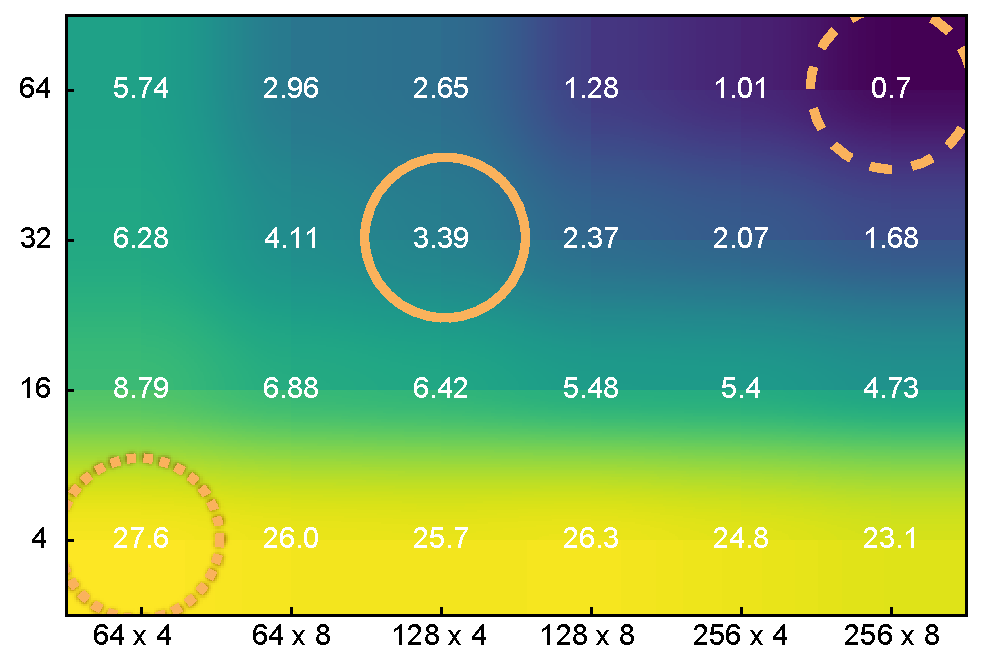
\includegraphics[width=0.48\linewidth]{TOG/figs/latency_vs_quality/heat_quality2.pdf}\label{fig:optimization:heat:quality}}
    \subfloat[latency]{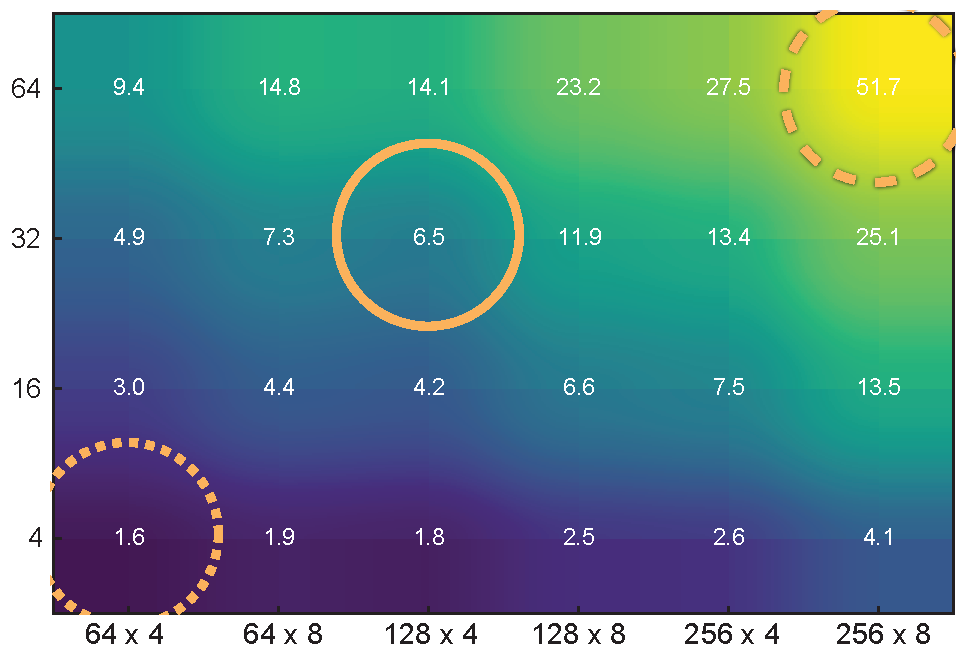
\includegraphics[width=0.48\linewidth]{TOG/figs/latency_vs_quality/heat_time2.pdf}\label{fig:optimization:heat:time}}
    
    \subfloat[quality-only]{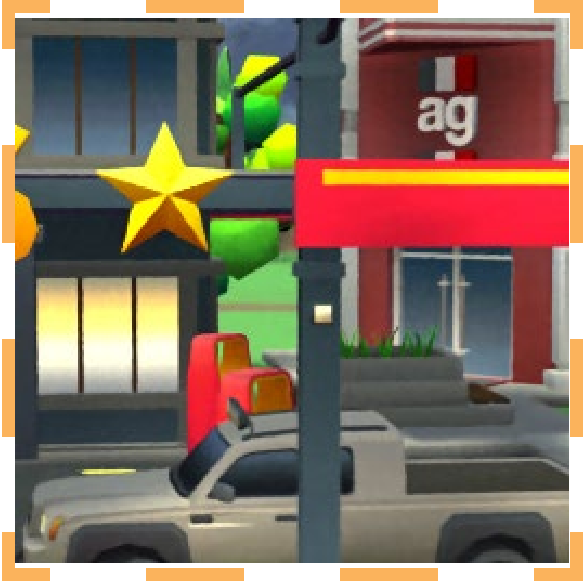
\includegraphics[width=0.3\linewidth]{TOG/figs/latency_vs_quality/quality_only.pdf}\label{fig:optimization:quality}}\hspace{0.5em}
    \subfloat[latency-only]{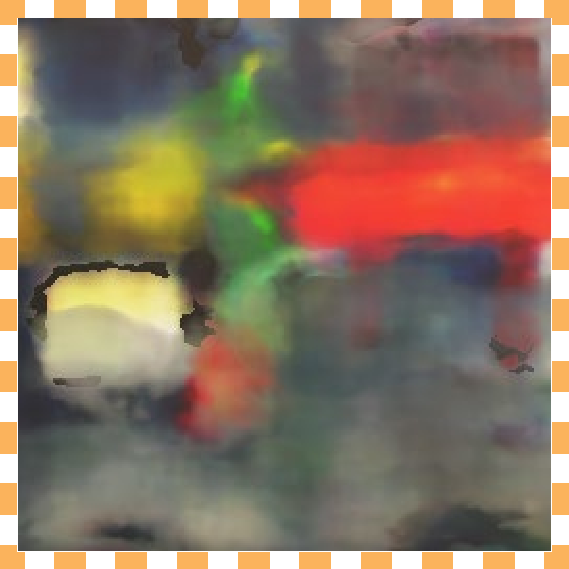
\includegraphics[width=0.3\linewidth]{TOG/figs/latency_vs_quality/latency_only.pdf}\label{fig:optimization:time}}\hspace{0.5em}
    \subfloat[ours]{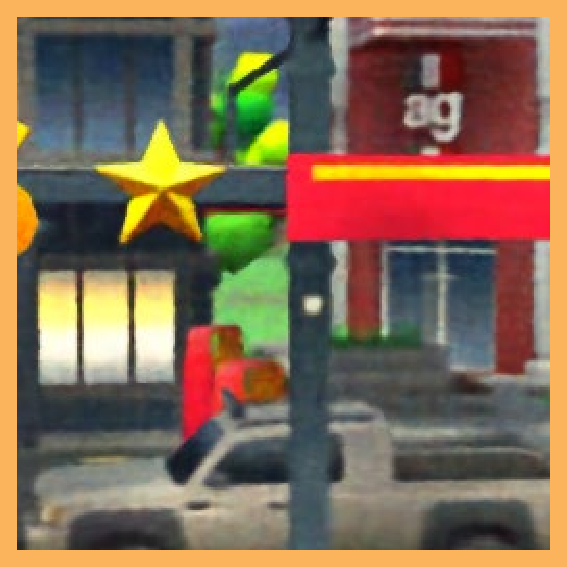
\includegraphics[width=0.3\linewidth]{TOG/figs/latency_vs_quality/our.pdf}\label{fig:optimization:our}}
    \Caption{Latency-quality joint-optimization.}
    {%
    \protect\subref{fig:optimization:heat:quality}/\protect\subref{fig:optimization:heat:time} shows \protect\Cref{eq:imageError}/latency(in millisecond under pytorch implementation) of an example foveal network.
    The values are computed with various settings of $\mlpLayerNum\times\mlpChannelNum$ (x-axis) and $\sphereNum$ (y-axis). The second row indicates a corresponding foveal image under different settings. Our method balances both perceptual quality and latency.\nothing{\qisun{(Jan 24) What is the unit of \subref{fig:optimization:heat:time}? It shouldn't be second, right?}\dnc{It's millisecond.}}%nothing
    }
    \label{fig:optimization}
\end{figure}
Inspired by \cite{Li:2020:TSP,albert2017latency}, we perform spatial-temporal joint modeling to determine the optimal coordinate system ($\sphereNum$) for positional precision and network complexity ($\mlpLayerNum$, $\mlpChannelNum$) for color precision that adapt to individual computational resources and scene content. This is achieved via latency-precision modeling in the spatial-temporal domain:
%Specifically, we model the prediction image $P$ with gaze position ($G$) at time $t$ as $P_G(t)$ and the ground truth retinal image (from a simulated local rendering) as $\hat{P}_G(t)$.
%In practice, increasing the number of spheres $\sphereNum$ or number of MLP layers may affect the computational and transmissional latency but will improve the quality of individual frames (as in \Cref{eq:imageError}). Thus, we define the perceptual error as:
\begin{equation}
\begin{aligned}
\finalError(\sphereNum, &\mlpLayerNum, \mlpChannelNum) = 
\sum_t\int \mlpFunc_{\mlpLayerNum, \mlpChannelNum}(\SpatialPt)\times\\ &\norm{\projectionMatrix(\rayo_t,\camDir_t)\cdot\SpatialPt-\projectionMatrix(\rayo_{t-\latency},\camDir_{t-\latency})\cdot\pt(\sphereRadius_k,\rayo_{t-\latency},\rayd_{t-\latency})}\mathbf{d}\SpatialPt,
%&\int  \norm{ \imgSpaceError(\sphereNum, \mathbf{\sphereRadius}, \rayo_t, \rayd_t) - \imgSpaceError(\sphereNum, \mathbf{\sphereRadius}, \rayo_{t-l(\sphereNum, \mathbf{\sphereRadius})}, \rayd_{t-l(\sphereNum, \mathbf{\sphereRadius})})) } \mathbf{d} t
\label{eq:error:image}
\end{aligned}
\end{equation}
where $\latency\triangleq\latency(\sphereNum, \mlpLayerNum, \mlpChannelNum)$ is the system latency with a given coordinate and network setting.
$\mlpFunc_{\mlpLayerNum, \mlpChannelNum}(\SpatialPt)$ is the four ($r,g,b,a$) output channels' L1-distance between a given network setting and the highest values $\sphereNum=64,\mlpLayerNum=8,\mlpChannelNum=256$). For simplicity, we assumed uniformly distributed $\mathbf{\sphereRadius}$ with a fixed range of the spherical coverage.%\zh{``and0 the highest values'' ??}

As suggested by Albert et al. \shortcite{albert2017latency}, the latency for a foveated system shall reach below \textasciitilde$50$ms for undetectable artifacts. Given our test device's eye-tracking latency \textasciitilde$12ms$ and the photon submission latency \textasciitilde$14ms$ (\cite{albert2017latency}), the synthesis and rendering latency shall be less than $L_0 = 24$ms.
Thus, we determine the optimal $\{\sphereNum, \mathbf{\sphereRadius}\}$ to balance latency and precision as
\begin{equation}
\begin{aligned}
    &\argmin_{\sphereNum, \mlpLayerNum, \mlpChannelNum} \finalError(\sphereNum, \mlpLayerNum, \mlpChannelNum), \\
    & s.t.\ {l(\sphereNum, \mathbf{\sphereRadius})} < L_0.
\end{aligned}
\end{equation}
\Cref{fig:optimization} visualizes an example of the optimization mechanism for an foveal image $\imageFoveal$. The optimized results ($\sphereNum, \mlpLayerNum, \mlpChannelNum$) for individual networks are used for training. The optimization outcomes are detailed in \Cref{sec:impl}.
The visual quality is validated by psychophysical study (\Cref{sec:study:user}) and objective analysis (\Cref{sec:study:quality}). The latency breakdown of our system is reported in \Cref{sec:study:intra}.
